
\documentclass [11pt,twoside]{article}
\usepackage[utf8]{inputenc}
\usepackage[T1]{fontenc}

%Page margins, header and footer positions
\usepackage{geometry}
 \geometry{
 a4paper,
 total={210mm,297mm},
 left=25mm,
 right=25mm,
 top=30mm,
 bottom=25mm,
 headsep=7mm}

\interfootnotelinepenalty=10000

%To display filling dots in the TOC for all entries
\usepackage[titles]{tocloft}
\renewcommand{\cftsecleader}{\cftdotfill{\cftdotsep}}

%Define new header and footer style
\usepackage{fancyhdr}

\pagestyle{fancy}
\fancyhf{}
\lhead{\color{Gray}{\small{S\&C project by CONTI, MARINO}}}
\lfoot{\textcolor{Gray}{\small{Copyright © 2024, CONTI, MARINO – All rights reserved}}}
\rfoot{\textcolor{Gray}{\thepage}}
\renewcommand{\headrulewidth}{0pt}

%PACKAGES
\usepackage{wasysym}
\usepackage{pifont}

\newcommand{\supported}{\ding{52}\xspace}
\newcommand{\unsupported}{\ding{55}\xspace}
\newcommand{\partsupported}{\textcolor{black!40}{\ding{52}}\xspace}
\newcommand{\lowsupported}{\textcolor{black!20}{\ding{52}}\xspace}
\newcommand{\unknowsupported}{\textbf{?}\xspace}

%Font: Times
\usepackage{times}
%Change monospaced font
\renewcommand{\ttdefault}{lmtt}

%tables
\usepackage{tabu}
\usepackage{tabularx}
\usepackage{ltablex}
\usepackage{longtable}
\usepackage{float} % To allow the use of H modifier in long tables

%landscape mode
\usepackage{pdflscape}
\usepackage{rotating}
\usepackage{caption}

%make landscape mode be sensitive to even and odd pages
%start
\def\myrotate{\ifodd\c@page\else-\fi 90}
\makeatletter
\global\let\orig@begin@landscape=\landscape%
\global\let\orig@end@landscape=\endlandscape%
\gdef\@true{1}
\gdef\@false{0}
\gdef\landscape{%
    \global\let\within@landscape=\@true%
    \orig@begin@landscape%
}%
\gdef\endlandscape{%
    \orig@end@landscape%
    \global\let\within@landscape=\@false%
}%
\@ifpackageloaded{pdflscape}{%
    \gdef\pdf@landscape@rotate{\PLS@Rotate}%
}{
    \gdef\pdf@landscape@rotate#1{}%
}
\let\latex@outputpage\@outputpage
\def\@outputpage{
    \ifx\within@landscape\@true%
        \if@twoside%
            \ifodd\c@page%
                \gdef\LS@rot{\setbox\@outputbox\vbox{%
                    \pdf@landscape@rotate{-90}%
                    \hbox{\rotatebox{90}{\hbox{\rotatebox{180}{\box\@outputbox}}}}}%
                }%
            \else%
                \gdef\LS@rot{\setbox\@outputbox\vbox{%
                    \pdf@landscape@rotate{+90}%
                    \hbox{\rotatebox{90}{\hbox{\rotatebox{0}{\box\@outputbox}}}}}%
                }%
            \fi%
        \else%
            \gdef\LS@rot{\setbox\@outputbox\vbox{%
                \pdf@landscape@rotate{+90}%
                \hbox{\rotatebox{90}{\hbox{\rotatebox{0}{\box\@outputbox}}}}}%
            }%
        \fi%
    \fi%
    \latex@outputpage%
}
\makeatother
%end

%graphics
\usepackage{graphicx}
\usepackage[dvipsnames, table]{xcolor}
%If you upload images from PC, you need to insert code for the path here (different for Windows and Unix OS)

%References
%\usepackage{xpatch}
%\usepackage[backend=biber, style=numeric, citestyle=numeric, sorting=none]{biblatex}
%\addbibresource{main.bib}

%Other
\usepackage{ifthen}
\usepackage{xspace}
\usepackage{enumitem}
\usepackage{amssymb}
\usepackage[pdftex, colorlinks]{hyperref}
\newcommand{\comment}[1]{{\color{Red}$\blacktriangleright$ Comment: #1 $\blacktriangleleft$}}


% Some utilities\ldots
\usepackage{soul}
\usepackage{tikz}

\usetikzlibrary{calc}
\usetikzlibrary{decorations.pathmorphing}


\makeatletter

\newcommand{\defhighlighter}[3][]{%
  \tikzset{every highlighter/.style={color=#2, fill opacity=#3, #1}}%
}

\defhighlighter{yellow}{.5}

\newcommand{\highlight@DoHighlight}{
  \fill [ decoration = {random steps, amplitude=1pt, segment length=15pt}
        , outer sep = -15pt, inner sep = 0pt, decorate
       , every highlighter, this highlighter ]
        ($(begin highlight)+(0,8pt)$) rectangle ($(end highlight)+(0,-3pt)$) ;
}

\newcommand{\highlight@BeginHighlight}{
  \coordinate (begin highlight) at (0,0) ;
}

\newcommand{\highlight@EndHighlight}{
  \coordinate (end highlight) at (0,0) ;
}

\newdimen\highlight@previous
\newdimen\highlight@current

\DeclareRobustCommand*\highlight[1][]{%
  \tikzset{this highlighter/.style={#1}}%
  \SOUL@setup
  %
  \def\SOUL@preamble{%
    \begin{tikzpicture}[overlay, remember picture]
      \highlight@BeginHighlight
      \highlight@EndHighlight
    \end{tikzpicture}%
  }%
  %
  \def\SOUL@postamble{%
    \begin{tikzpicture}[overlay, remember picture]
      \highlight@EndHighlight
      \highlight@DoHighlight
    \end{tikzpicture}%
  }%
  %
  \def\SOUL@everyhyphen{%
    \discretionary{%
      \SOUL@setkern\SOUL@hyphkern
      \SOUL@sethyphenchar
      \tikz[overlay, remember picture] \highlight@EndHighlight ;%
    }{%
    }{%
      \SOUL@setkern\SOUL@charkern
    }%
  }%
  %
  \def\SOUL@everyexhyphen##1{%
    \SOUL@setkern\SOUL@hyphkern
    \hbox{##1}%
    \discretionary{%
      \tikz[overlay, remember picture] \highlight@EndHighlight ;%
    }{%
    }{%
      \SOUL@setkern\SOUL@charkern
    }%
  }%
  %
  \def\SOUL@everysyllable{%
    \begin{tikzpicture}[overlay, remember picture]
      \path let \p0 = (begin highlight), \p1 = (0,0) in \pgfextra
        \global\highlight@previous=\y0
        \global\highlight@current =\y1
      \endpgfextra (0,0) ;
      \ifdim\highlight@current < \highlight@previous
        \highlight@DoHighlight
        \highlight@BeginHighlight
      \fi
    \end{tikzpicture}%
    \the\SOUL@syllable
    \tikz[overlay, remember picture] \highlight@EndHighlight ;%
  }%
  \SOUL@
}

\makeatother

% Common abbrev. are set as commands to ensure proper spacing after the dot
\RequirePackage{xspace}
\newcommand{\ie}{i.e.\@\xspace}
\newcommand{\aka}{a.k.a.\@\xspace}
\newcommand{\Ie}{I.e.\@\xspace}
\newcommand{\cf}{cf.\@\xspace}
\newcommand{\Cf}{Cf.\@\xspace}
\newcommand{\eg}{e.g.\@\xspace}
\newcommand{\Eg}{E.g.\@\xspace}
\newcommand{\etal}{et al.\@\xspace}
\newcommand{\etc}{etc.\@\xspace}
\newcommand{\wrt}{w.r.t.\@\xspace}
\newcommand{\Wrt}{W.r.t.\@\xspace}



\date{}

\usepackage{enumitem}
\usepackage[dvipsnames]{xcolor}
\usepackage{listings}
\usepackage{alloy-style}
\usepackage{float}

\begin{document}

%TITLE PAGE

\begin{titlepage}


%LOGO

{\begin{table}[t!]
\centering
\begin{tabu} to \textwidth { X[1.3,r,p] X[1.7,l,p] }
\textcolor{Blue}
{\textbf{\small{S\&C project by Conti, Marino}}} & 
\includegraphics[scale=0.5]{Images/PolimiLogo}
\end{tabu}
\end{table}}~\\ [7cm]

%TITLE 

\begin{flushleft}

%Replace the text string with your title
{\textcolor{Blue}{\textbf{\Huge{Requirement Analysis and Specification
        Document}}}} \\ [1cm]

\end{flushleft}

\end{titlepage}

%Define deliverable specific info
%Replace cell contents where needed
\begin{table}[h!]
\begin{tabu} to \textwidth { X[0.3,r,p] X[0.7,l,p] }
\hline

\textbf{Deliverable:} & RASD\\
\textbf{Title:} & Requirement Analysis and Verification Document \\
\textbf{Authors:} & Enzo Conti and María Marino \\
\textbf{Version:} & 1.0 \\ 
\textbf{Date:} & 22-December-2024 \\
\textbf{Download page:} & https://github.com/marinomaria/ContiMarino \\
\textbf{Copyright:} & Copyright © 2024, Conti, Marino – All rights reserved \\
\hline
\end{tabu}
\end{table}




\setcounter{page}{2}


%------------------------------------------------------------------------------------------------------------------------------------------------
\newpage
\addcontentsline{toc}{section}{Table of Contents}
\tableofcontents
\newpage
\addcontentsline{toc}{section}{List of Figures}
\listoffigures
\addcontentsline{toc}{section}{List of Tables}
\listoftables

%------------------------------------------------------------------------------------------------------------------------------------------------
\clearpage
{\color{Blue}{\section{Introduction}}}
\label{sect:introduction}
% This document has been prepared to help you approaching Latex as a formatting tool for your Travlendar+ deliverables. This document suggests you a possible style and format for your deliverables and contains information about basic formatting commands in Latex. A good guide to Latex is available here \href{https://tobi.oetiker.ch/lshort/lshort.pdf}{https://tobi.oetiker.ch/lshort/lshort.pdf}, but you can find many other good references on the web. 

% Writing in Latex means writing textual files having a \texttt{.tex} extension and exploiting the Latex markup commands for formatting purposes. Your files then need to be compiled using the Latex compiler. Similarly to programming languages, you can find many editors that help you writing and compiling your latex code. Here \href{https://beebom.com/best-latex-editors/}{https://beebom.com/best-latex-editors/} you have a short oviewview of some of them. Feel free to choose the one you like.  

% Include a subsection for each of the following items:
% \begin{itemize}
% \item
% Purpose: here we include the goals of the project
% \item
% Scope: here we include an analysis of the world and of the shared phenomena
% \item
% Definitions, Acronyms, Abbreviations
% \item
% Revision history
% \item
% Reference Documents 
% \item
% Document Structure
% \end{itemize}
% Below you see how to define the header for a subsection.


\subsection{Purpose}
As the demand for skilled professionals grows, facilitating smooth connections between students and companies becomes increasingly vital. Traditionally, students seeking internships often face challenges in finding opportunities that align with their skills and career goals, while companies struggle to identify the right talent. The Students\&Companies (S\&C) platform addresses this challenge by providing a space where university students and companies offering internships can easily find and connect with each other.

S\&C simplifies the process by matching students with internships based on their skills, experiences, and the opportunities offered by companies. The platform enhances the internship search and recruitment process, making it more efficient for both students looking to gain real-world experience and companies seeking fresh talent. By fostering better connections and streamlining communication, S\&C helps ensure that both students and companies can find the right fit, ultimately benefiting the growth of the workforce.
\subsubsection{Goals}
\begin{enumerate}[label={[G\arabic*]}]
    \item Students are able to look for internships and easily recognize the ones that matches their characteristics (skills, interests, experience).
    \item Companies are able to advertise their open internship projects and easily asses candidates' fit with them.
    \item Companies and students can have a well-defined, precise and concrete selection process.
    \item Through tailored recommendations, students can find suitable internships when those exist.
    \item Through tailored recommendations, companies can identify fitting candidates when those exist.
\end{enumerate}

\subsection{Scope}
In this section, we define the domain of the Students\&Companies (S\&C) platform, focusing on the main users and their interactions with the system. There are two primary user groups: Students and Companies.

Students are individuals enrolled in universities who use the platform to search for and apply to internship opportunities. They can create and manage their profiles, upload their CVs, and receive recommendations for internships that match their skills and preferences. Students can also proactively browse available internships, apply to them, and track the status of their applications.

Companies are organizations offering internships, using the platform to advertise available opportunities. They can post detailed internship descriptions, including tasks, benefits, and the skills required. Companies can also review student profiles, receive recommendations, and initiate the selection process, which may involve interviews and other assessments.

The platform facilitates a two-way interaction: students receive recommendations for internships that align with their qualifications, and companies can identify and reach out to students who fit their needs. Both students and companies can track the progress of their applications or listings and provide feedback to improve the matching process. Additionally, universities are involved in monitoring the internships, ensuring quality, and supporting students throughout the experience.
\subsubsection{World Phenomena}
\begin{enumerate}[label={[WP\arabic*]}]
    \item Students are interested in internship projects.
    \item Companies have internship positions to fill for projects.
    \item Each student has a set of characteristics (interest, skills, experience) organized in their CV that makes them fit or unfit for certain projects.
    \item Companies have a suited profile for each project and may have customized questionnaires that reflect this suited profile.
    \item Companies interview candidate students to asses their fit for the project.
    \item Once an internship is settled in it prescribes a set of responsibilities (workload, commitment, salary, environment) for both the student and the employer.
    \item Both parts individually keep track of each other's responsibilities and may have complaints about the other part action/behavior.
    \item When the internship ends, both parts may have feedback and suggestion regarding the whole process (interview, selection, development).
\end{enumerate}

\subsubsection{Shared Phenomena}
\begin{enumerate}[label={[SP\arabic*]}]
    \item[] \textbf{World controlled}
    \item Students provide information about their own characteristics.
    \item Companies provide a description, responsibilities and profile of the projects they offer.
    \item Companies upload customized questionnaires that structure their interviews.
    \item Companies submit feedback on interviews.
    \item Users report their complaints to S\&C.
    \item Users provide feedback and suggestions regarding past internships that can be relevant for future recommendations.
    \item[] \textbf{Machine controlled}
    \item Users receive notifications when relevant matching counterparts are available.
    \item During interviews, questionnaires become available to companies to collect students’ answers.
    \item Users communicate through the platform to set up a time and place for the interview.
    \item Students receive the company verdict about the interview process.
\end{enumerate}
\subsection{Definitions, Acronyms, Abbreviations}
\subsection{Revision history}
\subsection{Reference Documents}
This document is based on the following materials
\begin{itemize}
    \item R\&DD assignment specification of the Software Engineering II course a.a. 2024/5
    \item Slides of the same course available on WeBeep
\end{itemize}


\subsection{Document Structure}
\begin{itemize}
  \item \textbf{Introduction:} Brief description of the project, including its purpose, goals, and objectives.
  \item \textbf{Overall Description:} High-level overview of the system, explaining the involved phenomena and domain assumptions.
  \item \textbf{Specific Requirements:} Detailed analysis of requirements, including hardware and software constraints for developers.
  \item \textbf{Formal Analysis:} Formal description of world phenomena using Alloy.
  \item \textbf{Effort Spent:} Time spent on each section of the document.
  \item \textbf{References:} List of documents and software references used in the paper.
\end{itemize}


%------------------------------------------------------------------------------------------------------------------------------------------------
\clearpage
{\color{Blue}{\section{Overall Description}}}
\label{sect:overview}
% Here you can see how to include an image in your document.

% \begin{sidewaysfigure}
% \centering
% 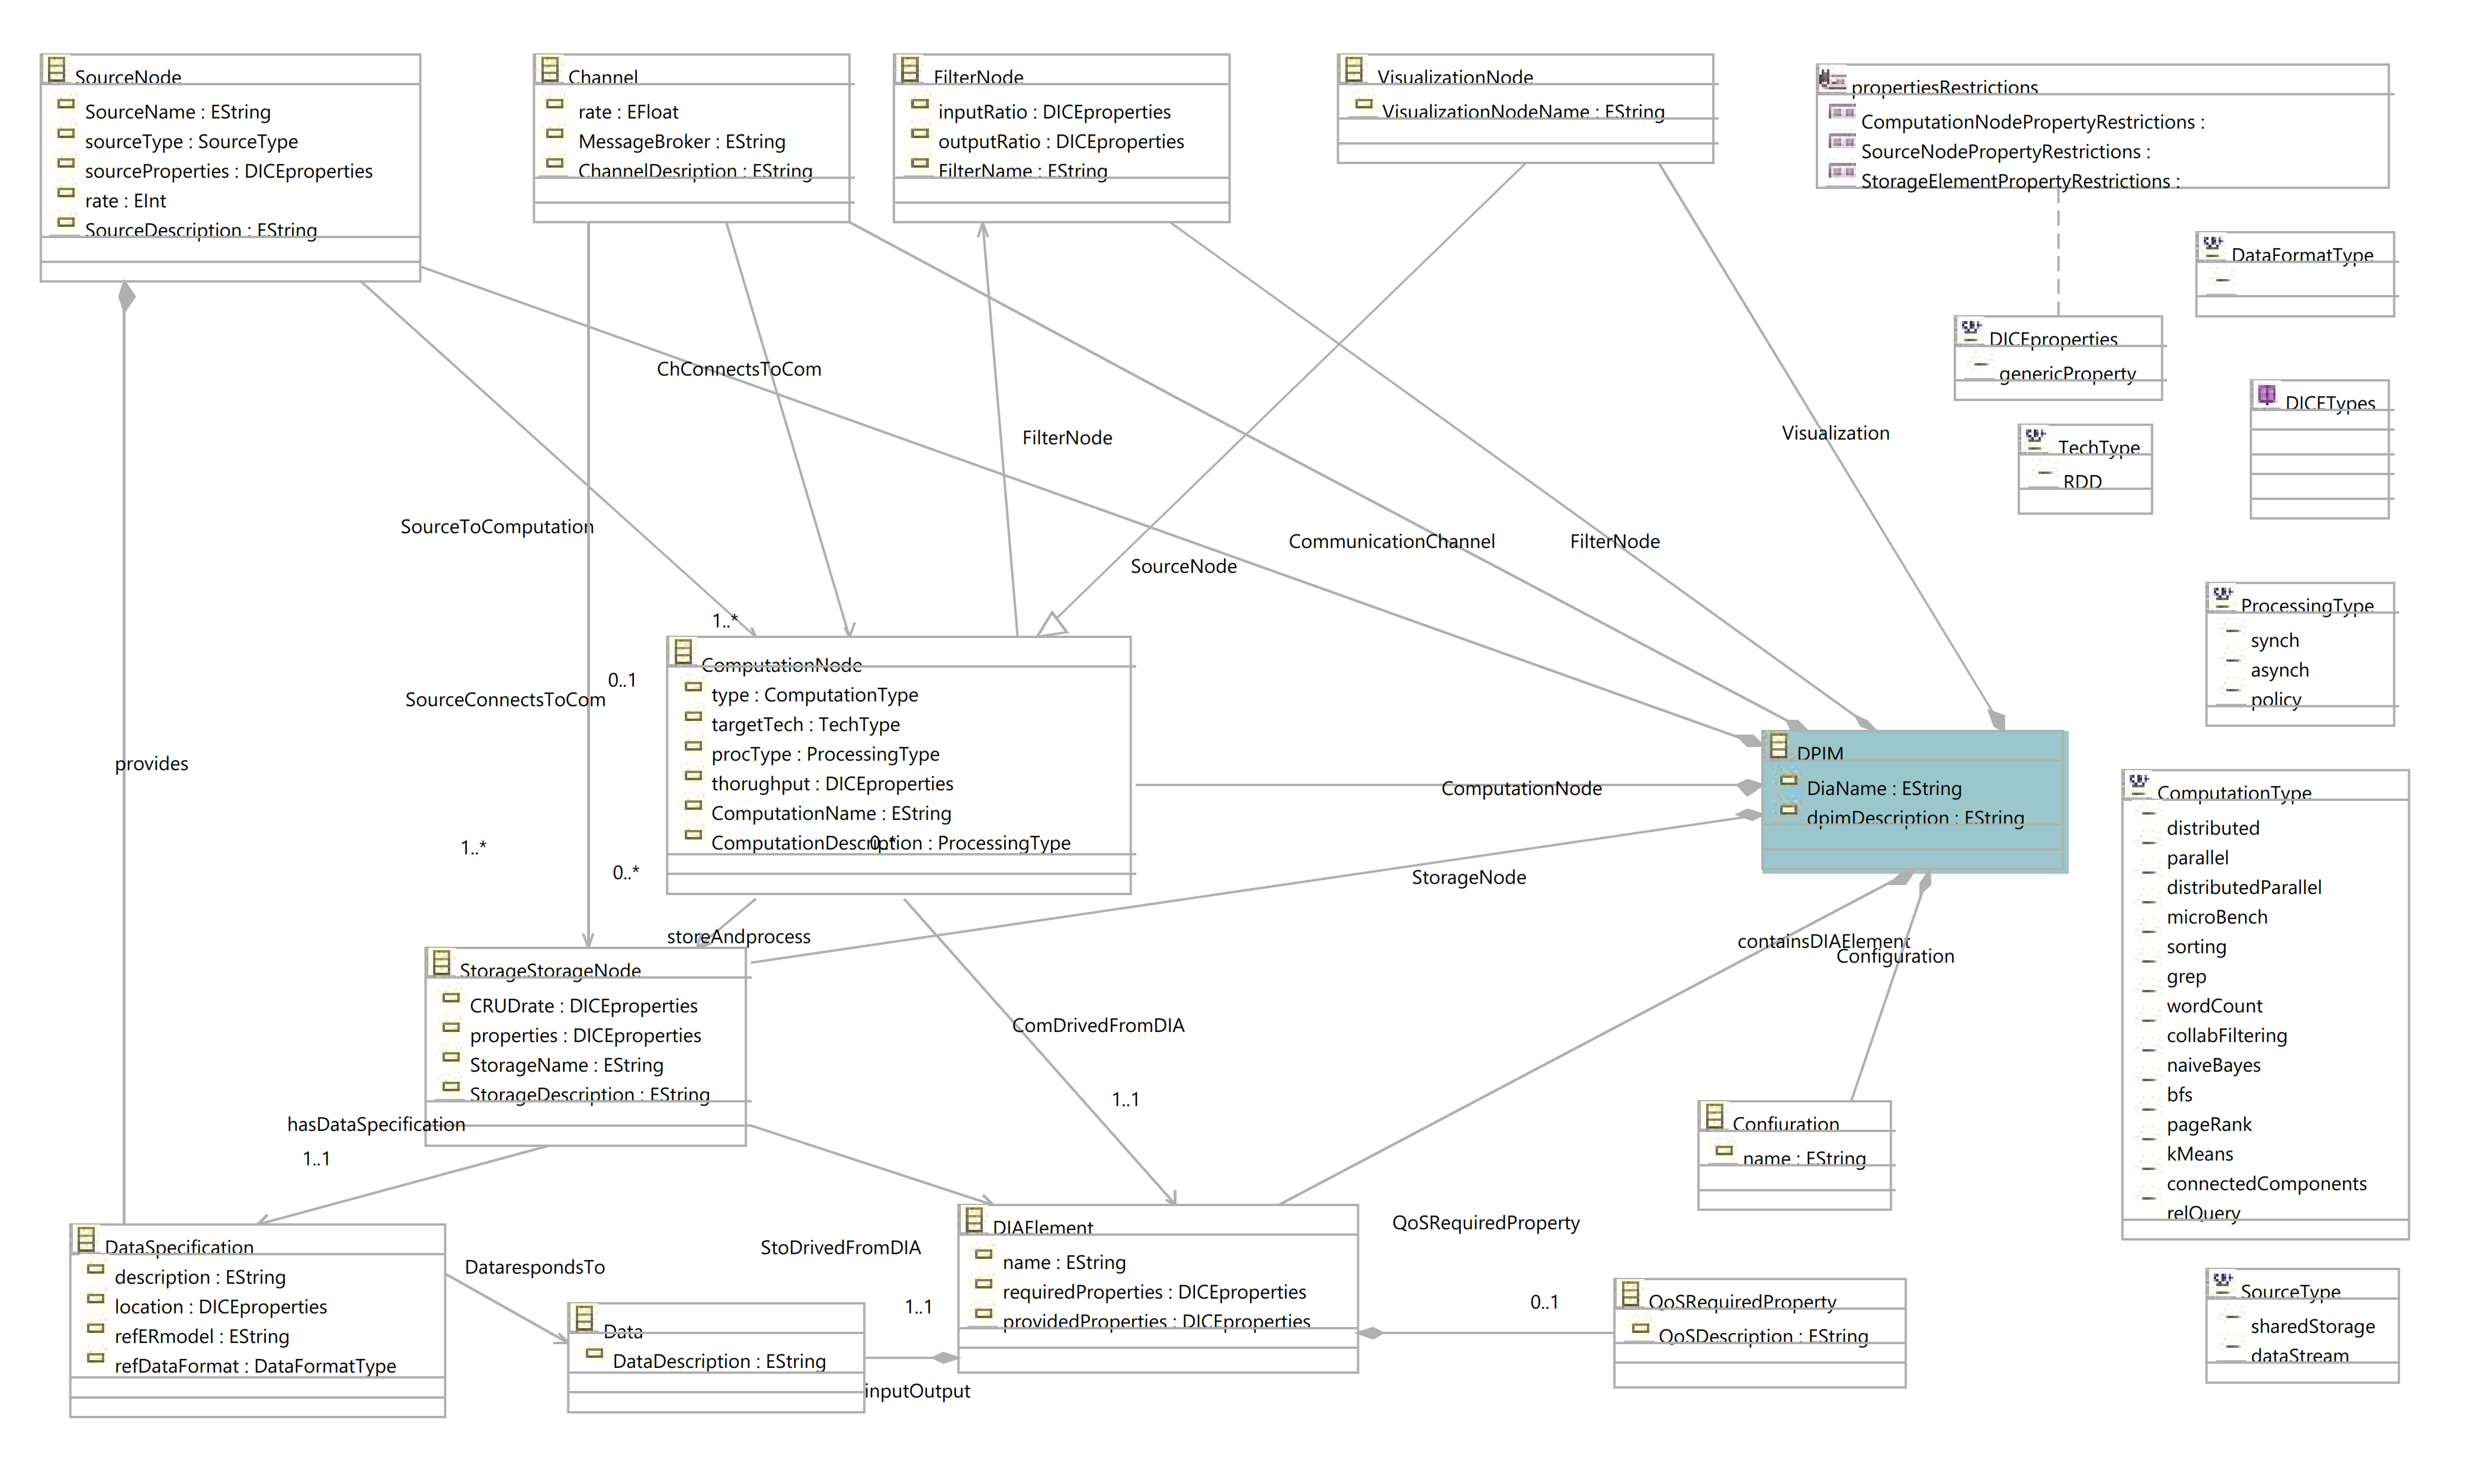
\includegraphics[width=\textwidth]{Images/11.png}
% \caption{\label{fig:metamodel}DICE DPIM metamodel.}
% \end{sidewaysfigure}

% \begin{figure}
% \centering
% 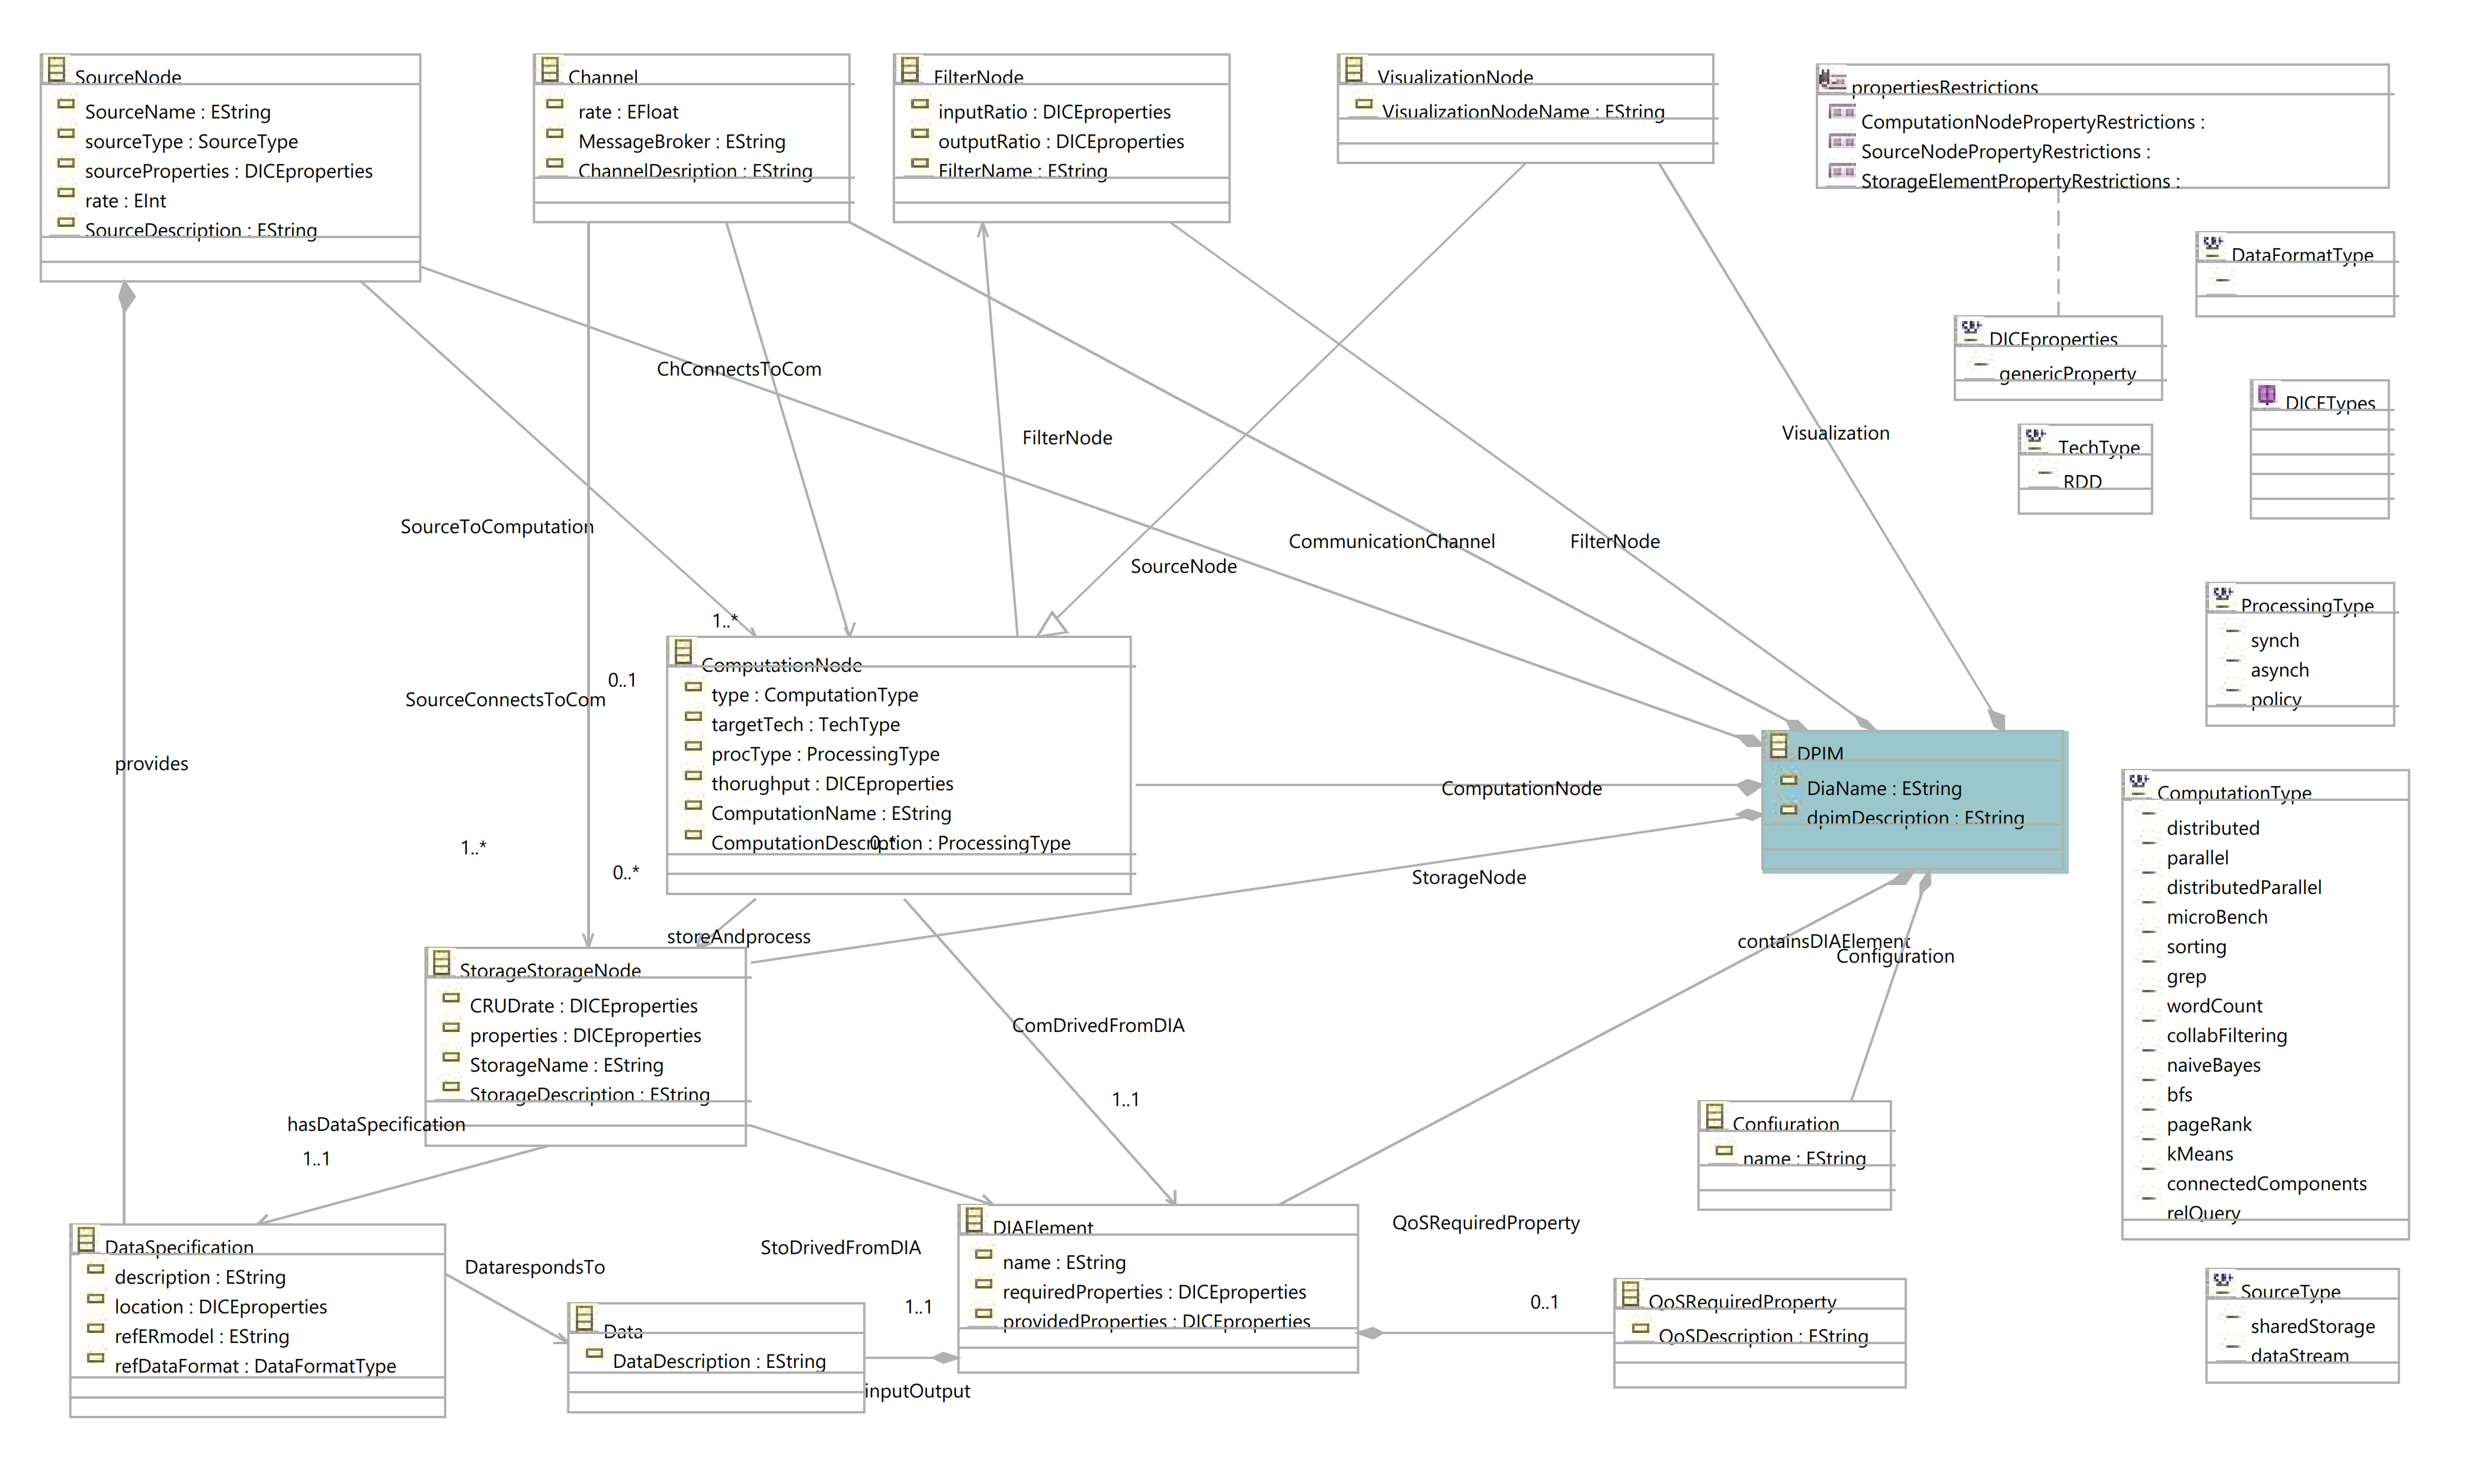
\includegraphics[width=\textwidth]{Images/11.png}
% \caption{\label{fig:metamodel2}DICE DPIM metamodel in portrait form.}
% \end{figure}

% Here is the command to refer to another element (section, figure, table, ...) in the document: \emph{As discussed in Section~\ref{sect:overview} and as shown in Figure~\ref{fig:metamodel}, ...}. Here is how to introduce a bibliographic citation~\cite{DAM}. Bibliographic references should be included in a \texttt{.bib} file. 

% Table generation is a bit complicated in Latex. You will soon become proficient, but to start you can rely on tools or external services. See for instance this \href{https://www.tablesgenerator.com}{https://www.tablesgenerator.com}. 
\subsection{Product Perspective}
\subsubsection{Scenarios}

\textbf{Student registers in the platform}

Dwight Schrute decides it's about time to get an internship, so he opens his notebook and acesses the S\&C website. Once acessed, the site offers a login page in which he clicks the ``New account'' button and is redirected to a page in which he fills his personal and contact information and uploads his CV. Once he is done with the form, S\&C checks the filling of all mandatory data, as well as the correctness of information (existing email, legal age, etc). A confirmation email is sent to his adress and, once confirmed, his account is registered and he can use it to login. Also, a profile is set to him according to his personal information and CV, which can be used later to recommendations.


\textbf{Publish new internship}

Toby, an HR representative at Dunder Mifflin Paper Company, is informed that the digitizations of assets project needs an intern. He meets up with the manager of the project to determine the requirements and responsibilities of the role. They also define the questionnaire interviewers will need to use to asses candidates during interviews. Then, he meets with the head of HR to refine the compensation package they will offer. With all the information, Toby navigates to S\&C in his browser. He logs in, clicks on ``New Internship Position'' and fills all the required details (skills, experience, compensation, benefits, duration and tasks-to-be-performed). Then he clicks the ``Save and Publish'' button. 

S\&C validates the inputted information. If it is not valid, it prompts Toby to correct it. Otherwise, it saves the position details and publishes the announcement. Toby sees a pop-up in his screen confirming that the position has been created successfully. 

 
\textbf{Cancel an open internship}

Francis is made aware by his boss that the internship position he’s looking to recruit for needs to be closed due to budget cuts in the company. He navigates to S\&C, logs in and clicks on ``Open internships''. There, he selects the aforementioned internship and clicks on ``Cancel Internship''. A pop-up appears on the screen asking for confirmation. He clicks on “Confirm”. 

 
\textbf{Student proactively looks for an internship}

Dwight opens the S\&C website to look for an internship. The website pops a login page, in which he enters his credentials and acesses the platform. Once logged in, he searches the internship of his dreams to better suit his needs, specifying filters such as work position, geographical location, available programs, companies of preference etc. He finds Dunder Mifflin Paper Company and clicks on one of their internship programs, expanding his view to all of the project’s provided information (duration, technologies used, benefits, payment…) in its main page. Given his enthusiasm on the internship offer, he clicks the easy-application button and S\&C register his application by adding him to the applicants poll. 

 
\textbf{S\&C matchmakes internships and students}

After the publication of Dunder Mifflin Paper Company internship position, S\&C runs its matching algorithm and finds a high suitability for Jim Halpert’s profile. He receives a notification email communicating him from the new opened position that might interest him and his account is added to the list of potential suitable profiles, available to Dunder Mifflin Paper Company.

 
 
\textbf{Schedule an interview}

Holly, the Hiring Manager of the Bomb Project at ACME, is notified through an email from S\&C that a new candidate applied for the internship she published two days ago. She then clicks on the link provided in the email and is redirected to the web-app S\&C, where she logs in and then reviews said candidate’s CV. She thinks the student might be a great fit for the role, so she clicks on the “Schedule an interview” button that appear right next to the candidate’s description.

A pop-up comes up prompting her to input her availability for the week and the desired interview duration for this candidate. She provides her schedule and clicks on “Save”.

 
\textbf{S\&C invites the candidate, Ryan, to an interview}

Ryan receives an email from S\&C inviting him to an interview for an internship he applied to. He clicks on the “Find a time” button. 

He is redirected to the S\&C website, where he logs in and is met with possible times for said interview. S\&C only shows the available times Holly provided. Ryan chooses Tuesday afternoon, as he does not have classes that day. He then clicks on “Confirm Assistance”.

S\&C schedules the interview and notifies the interviewer. Ryan is informed that his interview has been scheduled correctly.

\textbf{Carry on an interview}

Anna has an interview scheduled with Michael. He arrives on time to the office, Anna greets him and takes him to the conference room for the interview. She opens S\&C, logs in, and looks for the “Coffee Server Internship”, a customized questionnaire that her company uploaded to S\&C to conduct interviews for this role. She conducts her interview in her own style, rephrasing the questions from the questionnaire but extracting the key information. She takes notes of Michael’s answers and fills the questionnaire.

When Anna has all the information she needs to fill the questionnaire, she asks Michael if he has any questions. After he says no, she says goodbye and leads him to the exit. The interview finishes. Anna then goes back to her notes and reviews the questionnaire before saving it. When she clicks on “Save”, she is prompted to input a verdict (approve or reject) for Michael. The interview was good and Michael seemed really for for the role. She clicks on “Approve”. To submit the approval, S\&C asks her to provide the start date, time and place of the internship for Michael.

S\&C saves the interview as successful and notifies Michael about the good news. It also provides information about the start date, time and place of the internship.

 
    \textbf{Complain about an internship}

Gianna, the leader of the “Butterfly Effect” research project, is worried because the team is not getting along with the new intern. So she navigates to S\&C platform in her browser, logs in,  and clicks on the “Ongoing internships” tab. There, she selects the one that is causing trouble and then clicks on “Create Complaint”. A form pops-up asking her to provide a detailed description of the issue. She describes the issue and clicks on “Send”.

S\&C receives the complain and triggers a process involving the university to handle it (out of the project’s scope).

\textbf{The company provides a feedback to a finished internship}

John receives an email from S\&C asking for his feedback on past semester’s intern, Lorena. He is really happy with the work she’s done, and believes she might be a great fit for a full time position in the future. He clicks on the “Give feedback” button and is redirected to the S\&C app, where he logs in and is faced with four questions arranged on a form:

\begin{enumerate}
    \item How would you rate Lorena’s performance from one to ten?
    \item (Optional) Any comments on this internship in particular?
    \item (Optional) How would you rate your experience with S\&C from one to ten?
    \item (Optional) Any comments, feedback or suggestions on the platform?
\end{enumerate}

He fills the questionnaire and clicks on “Submit”

S\&C saves the data for statistical analysis.
 

\textbf{The student provides feedback to a finished internship}

Lorena receives an email from S\&C asking for her feedback on her recent internship at Dunder Mifflin. She is really happy with the experience and feels she learned a lot, especially in terms of project management and teamwork. She clicks on the “Give feedback” button and is redirected to the S\&C app, where she logs in and is faced with four questions arranged on a form:

\begin{enumerate}
    \item How would you rate your overall experience from one to ten?
    \item (Optional) Any comments on this internship in particular?
    \item (Optional) How would you rate your experience with S\&C from one to ten?
    \item (Optional) Any comments, feedback or suggestions on the platform?
\end{enumerate}

She fills out the questionnaire and clicks on “Submit.”

S\&C saves the data for statistical analysis.
\textbf{User looks at their analytics data}

Julian is preparing a mid-Q report on the hiring team’s performance. He opens the S\&C web-app, logs in and enters the “Analytics” tab. There, he is able to see three main metrics:

\begin{enumerate}
    \item Interest \%: Amount of students that applied over amount of students that saw an internship details for Julian’s company.
    \item Approval \%: Students that approved the interview over students that had interviews scheduled
    \item  Company NPS: Median feedback rate given to the company by students that completed internships position within it.
\end{enumerate}

He analyzes the metrics over time and takes a screenshot for a company presentation on the hiring processes.
\clearpage
\subsubsection{Domain Class Diagram}
\begin{figure}[H]
\centering
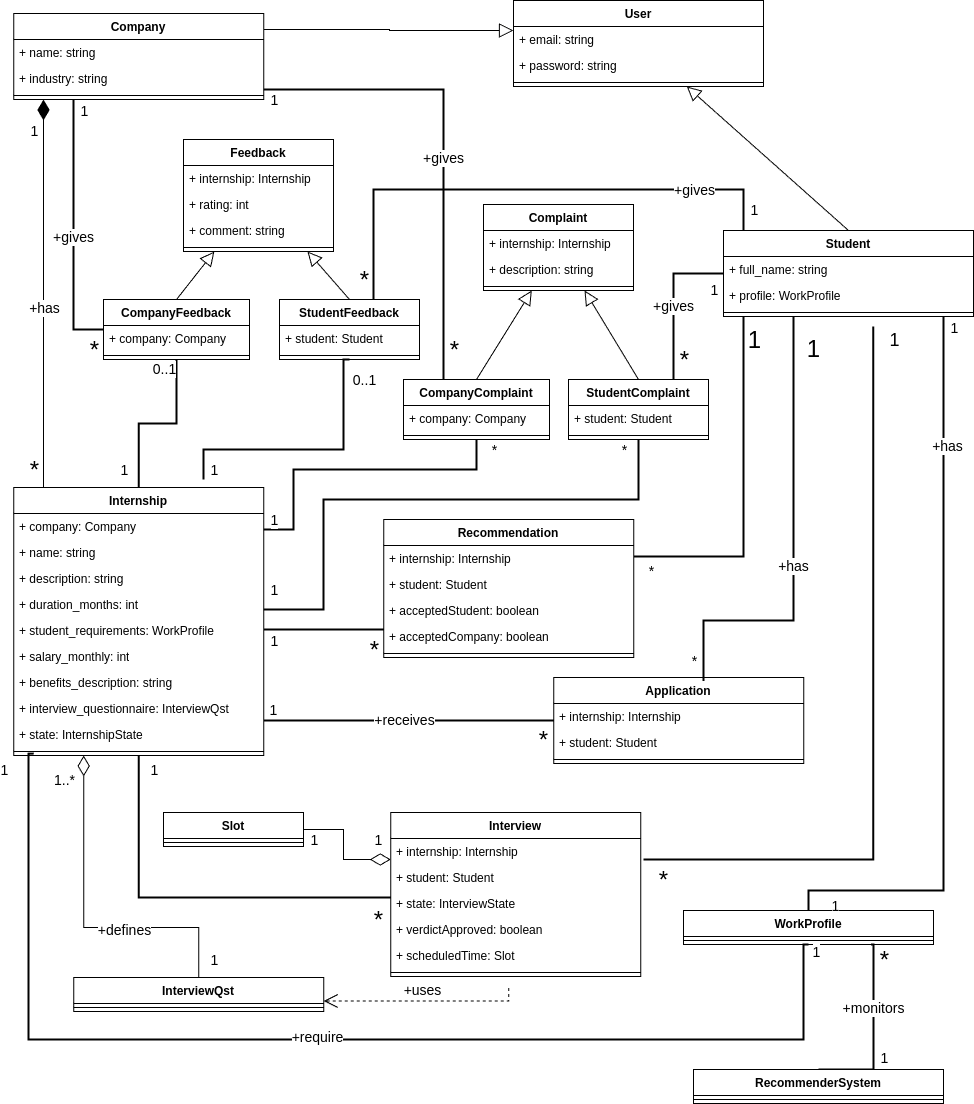
\includegraphics[scale=0.45]{Images/class-diagram.png}
\caption{\label{fig:class-diagram} Domain Level Class Diagram}
\end{figure}

\subsubsection{State Diagrams}

We chose to diagram interviews and internships because they are central entities in the selection process, representing its key stages. The states of these entities encapsulate the primary interactions between students and companies, making them essential to understand the overall workflow.

By focusing on these entities, we aimed to bring clarity to the reader by illustrating the core elements of the process. Their states naturally reflect the possible actions and outcomes, making them ideal candidates for state modeling and providing a structured view of the selection system.

\begin{figure}[H]
\centering
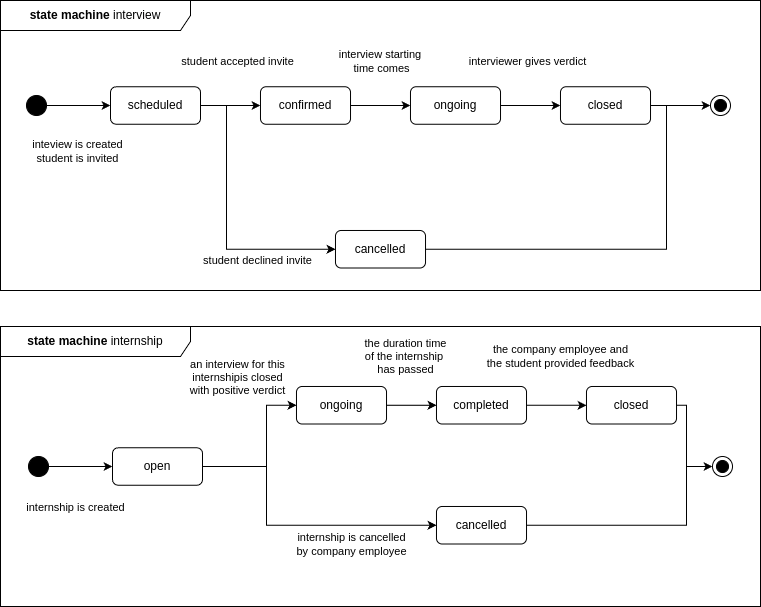
\includegraphics[width=\textwidth]{Images/state_diagrams.png}
\caption{\label{fig:state-diagrams} State Diagrams}
\end{figure}
\subsection{Product Functions}
\textbf{Sign-Up, Login, and Profile Management}

This function allows students and companies to sign up, log in, and manage their profiles on the platform. Upon signing up, students upload their CVs, which are used to create their profiles, while companies provide relevant organizational information. This function verifies the provided data (e.g., email, legal age) to ensure it meets platform requirements. Once registered, users can log in, update their information, and track their internship applications or postings.

\textbf{Internship Publication and Management}

This function allows companies to publish new internship positions, edit existing ones, and cancel open internships. Companies provide details such as required skills, tasks, compensation, and benefits, which are validated for correctness and completeness. Once published, the internship is visible to students. If necessary, companies can also manage ongoing internships by editing or canceling them, keeping the platform’s listings up to date.

\textbf{Search and Apply for Internships}

This function allows students to search for internships based on various criteria such as role, location, and compensation. Students can apply to internships with a single click, adding themselves to the list of applicants. The platform also sends proactive notifications to students about relevant opportunities, based on their profile data and past behaviors.

\textbf{Internship Matching and Recommendation}

This function allows the platform to recommend internships to students and suggest student profiles to companies based on matching criteria. The matching algorithm evaluates student profiles and internship details to suggest suitable opportunities. It continuously refines recommendations using data from student interactions (such as applications) and feedback from companies. The system sends notifications to both parties about suitable internships or candidates.

\textbf{Interview Management and Selection Process}

This function allows companies to schedule interviews with students, manage interview details, and track candidate progress. Companies provide available time slots, and students confirm their attendance. During interviews, companies use custom questionnaires to assess candidates, recording feedback in the platform. Afterward, companies decide whether to approve or reject candidates, and the platform tracks the outcome, notifying both parties about the decision.

\textbf{Feedback and Complaint Management}

This function allows students and companies to provide feedback on internship experiences and raise complaints during ongoing internships. After internships conclude, companies rate students' performance, while students rate their overall experience. The platform uses this feedback to improve future internship matches. If issues arise during an internship, either students or companies can file complaints, which are then handled by the platform, often involving university representatives for resolution.

\textbf{Internship Analytics and Reporting}

This function allows companies and the platform to track and analyze various metrics related to internships. Metrics such as application rates, interview success rates, and feedback scores are collected to evaluate and improve the internship process. This data also feeds into the recommendation system, enhancing the quality of future matches between students and internships. Companies can view performance reports and adjust their recruitment strategies accordingly.
\subsection{User characteristics}

\textbf{Student}

The student is a user who creates and manages their profile, including uploading their CV, providing personal and academic details, and specifying internship preferences. Students can search for available internships, apply to positions, and receive notifications about opportunities that match their profiles. They can view internship details, track their applications, and receive interview invitations. After completing an internship, students can provide feedback on their experience and file complaints about ongoing internships if needed. Based on their profiles and activities, students are matched with relevant internship opportunities through the platform’s recommendation system. The student’s role focuses on searching for, applying to, and managing internship applications, participating in interviews, and engaging in feedback processes.

\textbf{Company}

The company user can create and manage their organizational profile, as well as publish internship listings. They provide details such as required skills, tasks, compensation, benefits, and other terms. Companies can edit, cancel, or close internship listings as necessary. They are responsible for reviewing student applications, selecting candidates, scheduling interviews, and conducting interviews using custom questionnaires. Once an internship is completed, companies can provide feedback on the student’s performance. Companies also have the option to file complaints about ongoing internships if issues arise. Additionally, they can access analytics to monitor the recruitment process, track key metrics like application success rates, interview outcomes, and student feedback, and evaluate the overall performance of their internship programs.
\subsection{Assumptions, Dependencies and Constraints}
\subsubsection{Domain Assumptions}
    \begin{enumerate}[label={[DA\arabic*]}]
        \item Users provide accurate and up-to-date information to the platform.
        \item Students have a CV and a notion of their skills and profile.
        \item Companies have a detailed notion of the internship position and the profile they are hiring for.
        \item Internships are temporal contracts with explicit deadlines .
        \item Companies have a pre-defined process for hiring that involves interaction with S\&C.
        \item The company user sticks to the company-defined hiring process through the platform.
        \item Users interested in setting-up interviews know in advance their availability for the week.
        \item Every user has a valid email account that they check at least once every 48 hours.
        \item Email communication is regarded by users as a reliable channel for work-related information.
        \item Students are proactively interested in getting an internship.
        \item Users remember their authentication credentials
    \end{enumerate}


%------------------------------------------------------------------------------------------------------------------------------------------------
\clearpage
{\color{Blue}{\section{Specific Requirements}}}
\label{sect:requirements}
\subsection{External Interface Requirements}
\subsubsection{User Interfaces}
\subsubsection{Hardware Interfaces}
The Students\&Companies (S\&C) platform is a web-based application, so it does not require any specific hardware interface. It is accessible via computers, smartphones, or any other device with a web browser and an internet connection.
\subsubsection{Software Interfaces}
\begin{itemize}
    \item \textbf{Recommendation Engine API} To provide internship recommendations to students based on their profiles, skills, and previous interactions.
    \item \textbf{Email Notification Service} To send notifications to students and companies about internship opportunities, application statuses, and important deadlines.
\end{itemize}
\subsubsection{Communication Interfaces}
The platform requires an active internet connection to allow users to interact with it. Communication between users within the platform is done via messaging and notification systems. Students and companies can also use the platform to exchange information regarding internships, applications, and interviews.

The platform must be HTTPS compliant to ensure secure communication between users and the platform itself, protecting user data and interactions.




\subsection{Functional Requirements}

\begin{enumerate}[label={[R\arabic*]}]
\item[] \textbf{Sign-Up, Login, and Profile Management}


\item The system should provide authentication so that each action can be correctly associated with a user


\item When a student registers the system generates a profile containing their experience, skills, and education


\item[] \textbf{Internship Publication and Management}


\item The system allows companies to create new internship positions at any time


\item When a company user clicks on “create internship”, the system prompts the company for all the required information and checks its validity before saving


\item When an internship is successfully created, the system generates a work profile containing the required experience and skills for the position

 
\item When and internship is successfully created it should be findable through the search internship feature and allow student applications

\item[] \textbf{Search and Apply for Internships}


\item When a student searches for an internship through the platform, the system accurately processes the student’s search criteria to display related internships


\item When an internship is selected, the system’s user interface summarizes internship information


\item When a student searches for an internship through the platform, the displayed internships  are within the selected filters


\item When a student searches for an internship through the platform, the displayed internships are ordered accordingly to the field specified in student’s criteria

\item The system shall allow students to apply to the displayed internship without adding additional information


\item When the application button is clicked, the system shall save the student information and profile and notify the company

\item[] \textbf{Internship Matching and Recommendation}


\item The system shall provide regular monitoring to all stored profiles from students and internships


\item The system shall attempt to match student profiles with internship profiles


\item In every match found between an internship and a student, the system shall notify both parts about it


\item The matching algorithm used to find recommendations is accurate and can be improved through user feedback

\item[] \textbf{Interview Management and Selection Process}


\item The system allows company users to review any student profile


\item The system allows company users to invite any student to an interview


\item The system notifies the company when there are new student profiles to review (either applied or recommended)


\item When the company user clicks on “invite to interview” over a student, the system prompts the company user to provide possible availability slots for that specific interview

 
\item When the company user creates an interview by providing their availability the system notifies the selected student in less than 6 hours after the interview creation


\item The system allows students to decline the interview they have been invited for

 
\item If the student does not reply to the interview invitation after 48 hours from the sending time, the system declines the interview automatically


\item When a student accepts an interview invite, the system prompts them to select one of the available time slots for having the interview


\item The system does not allow the student to accept an interview invite without selecting one of the available slots the system provides


\item When the interview starting time comes (slot start), the system provides the company user with the questionnaire associated with the internship the interview is for


\item When the interview finishing time comes (slot end), the system prompts the company user for an interview verdict (approve or reject)


\item When the company user rejects the student after an interview, the system notifies the student


\item When the company user approves the student after an interview, the system prompts them to provide the start time and place of the internship


\item The system does not allow the company to approve the student without providing the internship start time and place


\item When a company user approves the student after an interview, the system notifies the student of the start time and place of the internship

\item[] \textbf{Feedback and Complaint Management}

\item When the duration time of an internship has passed since its starting time, the system notifies and prompts both the company user and the student to provide feedback on the internship experience


\item The system will not allow any user to use other features of the platform (besides login and feedback) when they have pending feedback on past internships

 
\item When a user provides feedback on an internship the system notifies its counterpart in the internship about the received feedback


\item The system allows any user to create a complaint about any of their ongoing internships

 
\item When a user creates a complaint the system prompts them to provide a non-empty description of the issue

\end{enumerate}

\subsubsection{Use Cases}
\textbf{UC1: Form Filling} (Table \ref{tab:UC1})
\begin{table}[H]
\centering
\caption{\textbf{UC1: Form Filling}}
\label{tab:UC1}
\resizebox{\textwidth}{!}{%
\begin{tabular}{|c|l|}
\hline
\textbf{Actors}           & user                                                       \\ \hline
\textbf{Entry Condition}   & an empty form is displayed on the user’s screen. the user knows all the required information. \\ \hline
\textbf{Event Flow}        & 1. the user completes the form with the required information \\
                           & 2. the user clicks on the “Submit” button                   \\
                           & 3. S\&C validates the inputted information and stores it in its internal database. \\ \hline
\textbf{Exit Condition}    & the data is correctly stored in the system’s internal database. \\ \hline
\textbf{Exceptions}        & the system detects that some of the provided information is invalid or empty.  \\ & it shows an error to the user and prompts them to correct it. \\ \hline
\end{tabular}
}
\end{table}

\textbf{UC2: Register Student }(Table \ref{tab:UC2})
\begin{table}[H]
\centering
\caption{\textbf{UC2: Register Student}}
\label{tab:UC2}
\begin{tabularx}{\textwidth}{|X|X|}
\hline
\textbf{Actors}           & student                                                   \\ \hline
\textbf{Entry Condition}   & the user has opened the S\&C Website and has all the required information. \\ \hline
\textbf{Event Flow}        & 1. S\&C Website initial page prompts the user to identify  \\
                           & 2. The user presses the “New Account” button             \\
                           & 3. S\&C shows a form to be completed with:               \\
                           & \hspace{1em} a. Email                                      \\
                           & \hspace{1em} b. Password                                   \\
                           & \hspace{1em} c. Full Name                                 \\
                           & \hspace{1em} d. Skills, interests, experience, education… \\
                           & 4. Included use case: form filling                        \\ \hline
\textbf{Exit Condition}    & A student is properly registered and has a valid account. \\ \hline
\textbf{Exceptions}        & none                                                      \\ \hline
\end{tabularx}
\end{table}

\textbf{UC3: Register Company }(Table \ref{tab:UC3})
\begin{table}[H]
\centering
\caption{\textbf{UC3: Register Company}}
\label{tab:UC3}
\begin{tabularx}{\textwidth}{|X|X|}
\hline
\textbf{Actors}           & company employee                                         \\ \hline
\textbf{Entry Condition}   & the company employee has opened the S\&C Website and has all the required information. \\ \hline
\textbf{Event Flow}        & 1. S\&C Website initial page prompts the company employee to identify  \\
                           & 2. The company employee presses the “New Account” button             \\
                           & 3. S\&C shows a form to be completed with:                          \\
                           & \hspace{1em} a. Email                                             \\
                           & \hspace{1em} b. Password                                          \\
                           & \hspace{1em} c. Company Name                                      \\
                           & \hspace{1em} d. Industry                                          \\
                           & 4. Included use case: Form Filling                                 \\ \hline
\textbf{Exit Condition}    & A company is properly registered and has a valid account.        \\ \hline
\textbf{Exceptions}        & none                                                           \\ \hline
\end{tabularx}
\end{table}

\textbf{UC4: User Login }(Table \ref{tab:UC4})
\begin{table}[H]
\centering
\caption{\textbf{UC4: User Login}}
\label{tab:UC4}
\begin{tabularx}{\textwidth}{|X|X|}
\hline
\textbf{Actors}           & user                                                       \\ \hline
\textbf{Entry Condition}   & the user has opened the S\&C Website and knows their credentials. \\ \hline
\textbf{Event Flow}        & 1. S\&C Website initial page prompts the user to identify  \\
                           & 2. The user clicks on the “Log In” button                   \\
                           & 3. S\&C shows a form to be completed with:                  \\
                           & \hspace{1em} a. Email                                        \\
                           & \hspace{1em} b. Password                                     \\
                           & 4. Included use case: Form Filling                           \\ \hline
\textbf{Exit Condition}    & User is logged into the platform.                           \\ \hline
\textbf{Exceptions}        & none                                                        \\ \hline
\end{tabularx}
\end{table}

\textbf{UC5: Search Internship }(Table \ref{tab:UC5})
\begin{table}[H]
\centering
\caption{\textbf{UC5: Search Internship}}
\label{tab:UC5}
\begin{tabularx}{\textwidth}{|X|X|}
\hline
\textbf{Actors}           & student                                                   \\ \hline
\textbf{Entry Condition}   & The student is logged into S\&C platform.                  \\ \hline
\textbf{Event Flow}        & 1. S\&C main page shows a search tab with filters            \\
                           & 2. Student taps the search bar and specifies the relevant information by either keywords or filters (company name, duration, …) \\
                           & 3. S\&C shows a list of matching available internships      \\
                           & 4. Student scrolls through her/his options and compares them as he/she wills \\
                           & 5. Student clicks on a specific internship opportunity      \\
                           & 6. S\&C shows the internship’s details                      \\ \hline
\textbf{Exit Condition}    & Student has performed the search and knows more about the internships he/she can apply to \\ \hline
\textbf{Exceptions}        & There is no matching result for the search. S\&C throws a “no results” page and suggests the user to alter filters. \\ \hline
\end{tabularx}
\end{table}

\textbf{UC6: Apply Internship }(Table \ref{tab:UC6})
\begin{table}[H]
\centering
\caption{\textbf{UC6: Apply Internship}}
\label{tab:UC6}
\begin{tabularx}{\textwidth}{|X|X|}
\hline
\textbf{Actors}           & student                                                   \\ \hline
\textbf{Entry Condition}   & The student is logged into S\&C platform and currently in a specific internship’s main page \\ \hline
\textbf{Event Flow}        & 1. Along with the internship details, the internship offer main page shows an “easy-apply” button \\
                           & 2. The user clicks the button willing to apply for it       \\
                           & 3. S\&C registers their application, shows a page of “Application Successful” and informs the student that he/she is going to receive feedback in 1 month at worst \\ \hline
\textbf{Exit Condition}    & Student has applied successfully to an internship position \\ \hline
\textbf{Exceptions}        & none                                                      \\ \hline
\end{tabularx}
\end{table}



\textbf{UC7: New Recommendation }(Table \ref{tab:UC7})
\begin{table}[H]
\centering
\caption{\textbf{UC7: New Recommendation}}
\label{tab:UC7}
\begin{tabularx}{\textwidth}{|X|X|}
\hline
\textbf{Actors}           & RecommenderSystem                                         \\ \hline
\textbf{Entry Condition}   & There exists at least one student and one internship, both properly registered in the system, it’s the time where the recommender system is scheduled \\ \hline
\textbf{Event Flow}        & 1. RecommenderSystem scans S\&C’s database via API \\
                           & 2. RecommenderSystem outputs a list of recommendations and posts them to S\&C (API call) \\
                           & 3. Included Use case: Send Notification. S\&C receives the recommendations and for each one of them it \\
                           & 4. S\&C sends a notification to the student about the new internship suggestion and a link to apply immediately. \\ \hline
\textbf{Exit Condition}    & The student is aware of a new internship option and is informed about it with an actionable link \\ \hline
\textbf{Exceptions}        & The RecommenderSystem does not generate any valid matches.  \\ \hline
\end{tabularx}
\end{table}

\textbf{UC8: New Internship }(Table \ref{tab:UC8})
\begin{table}[H]
\centering
\caption{\textbf{UC8: New Internship}}
\label{tab:UC8}
\begin{tabularx}{\textwidth}{|X|X|}
\hline
\textbf{Actors}           & company employee                                         \\ \hline
\textbf{Entry Condition}   & The company employee is logged in and knows all the detail about the internship position he/she wants to create \\ \hline
\textbf{Event Flow}        & 1. The company employee clicks on “New Internship Position”  \\
                           & 2. S\&C shows a form to be completed with the relevant information: \\
                           & \hspace{1em} a. Internship Position Name                    \\
                           & \hspace{1em} b. Internship Position Requirements (skills, previous experience…) \\
                           & \hspace{1em} c. Internship Position Description (Project, tasks to be performed) \\
                           & \hspace{1em} d. Internship Position Compensation & Benefits \\
                           & \hspace{1em} e. Internship Position Duration               \\
                           & \hspace{1em} f. Internship Position Customized Questionnaire for Interviews \\
                           & 3. Included Use Case: form filling \\
                           & 4. S\&C saves the new internship position in its internal database, publishes it and informs the company employee that the position has been created successfully \\ \hline
\textbf{Exit Condition}    & A new internship position is created successfully.       \\ \hline
\textbf{Exceptions}        & none                                                      \\ \hline
\end{tabularx}
\end{table}

\textbf{UC9: Cancel Internship }(Table \ref{tab:UC9})
\begin{table}[H]
\centering
\caption{\textbf{UC9: Cancel Internship}}
\label{tab:UC9}
\begin{tabularx}{\textwidth}{|X|X|}
\hline
\textbf{Actors}           & company employee                                         \\ \hline
\textbf{Entry Condition}   & The company employee is logged in and there’s an open internship for the company \\ \hline
\textbf{Event Flow}        & 1. The company employee clicks on “Open Internships”         \\
                           & 2. A list of open internships appear, he/she clicks on the internship he/she wants to cancel \\
                           & 3. He/she clicks on “Cancel Internship”                     \\
                           & 4. S\&C shows a pop-up asking for confirmation, he/she then clicks on confirm \\
                           & 5. S\&C changes the internship state to “cancelled”, stops showing it in the searches nor recommendations, and no longer receives applications. \\ \hline
\textbf{Exit Condition}    & The desired internship position is cancelled.             \\ \hline
\textbf{Exceptions}        & none                                                      \\ \hline
\end{tabularx}
\end{table}

\textbf{UC10: Schedule Interview }(Table \ref{tab:UC10})
\begin{table}[H]
\centering
\caption{\textbf{UC10: Schedule Interview}}
\label{tab:UC10}
\begin{tabularx}{\textwidth}{|X|X|}
\hline
\textbf{Actors}           & company employee, student                                \\ \hline
\textbf{Entry Condition}   & Company employee is interested in scheduling an interview with a student (either recommended or applied). Both actors are properly registered. The company employee is logged into the platform. \\ \hline
\textbf{Event Flow}        & 1. The company employee clicks on “Schedule an Interview” next to a student’s name or in a notification. \\
                           & 2. S\&C prompts her to input her availability for the next week, desired interview duration and position they’re interviewing for if they have more than one opened at the moment (Included Use Case: form filling) \\
                           & 3. S\&C receives the scheduling request and sends an email to the student, inviting them to the first available slot from the ones provided by the company employee (Included Use Case: send notification) \\
                           & 4. The student opens the email and clicks on the Find a Time button \\
                           & 5. (Included Use Case: user login) \\
                           & 6. Student is prompted to select one of the available slots for interview, then to confirm his/her selection \\
                           & 7. S\&C saves the interview in its internal database and notifies the interviewer (Included Use Case: send notification). \\ \hline
\textbf{Exit Condition}    & A new interview is scheduled correctly and stored in the system’s database. \\ \hline
\textbf{Exceptions}        & The student cannot assist in any of the available slots or is not interested. He clicks on the “Decline” button and is redirected to the main page. No interview is created. \\ \hline
\end{tabularx}
\end{table}

\textbf{UC11: Process Interview }(Table \ref{tab:UC11})
\begin{table}[H]
\centering
\caption{\textbf{UC11: Process Interview}}
\label{tab:UC11}
\begin{tabularx}{\textwidth}{|X|X|}
\hline
\textbf{Actors}           & company employee, student                                \\ \hline
\textbf{Entry Condition}   & There’s an interview scheduled between a company employee and a student. Both actors are properly registered, the company employee is logged into the platform. \\ \hline
\textbf{Event Flow}        & 1. The company employee clicks on “Start Interview” \\
                           & 2. S\&C shows the customized questionnaire associated with the internship position the company is interviewing for \\
                           & 3. Included Use Case: form filling \\
                           & 4. The company employee either approves or rejects the candidate when prompted \\
                           & \hspace{1em} a. If he/she approves the candidate, S\&C asks them to provide start date, time and place of the internship (Included Use Case: form filling) \\
                           & 5. S\&C saves the interview verdict and information. \\
                           & 6. S\&C sends a notification to the student with the verdict and, only if approved, the start date, time and place of the internship. \\ \hline
\textbf{Exit Condition}    & The interview is closed with a verdict and stored in the system’s database. \\ \hline
\textbf{Exceptions}        & The student doesn’t show up. In that case, the company employee can click on the “No Show” button in the questionnaire, and the candidate is rejected automatically. \\ \hline
\end{tabularx}
\end{table}

\textbf{UC12: New Complaint }(Table \ref{tab:UC12})
\begin{table}[H]
\centering
\caption{\textbf{UC12: New Complaint}}
\label{tab:UC12}
\begin{tabularx}{\textwidth}{|X|X|}
\hline
\textbf{Actors}           & user                                                       \\ \hline
\textbf{Entry Condition}   & There’s an ongoing internship involving the user. The user is registered and logged into the platform. \\ \hline
\textbf{Event Flow}        & 1. User clicks on “Ongoing Internships” in the website menu and then selects the internship he/she wants to complain about \\
                           & 2. Then, he/she clicks on “Create Complaint” \\
                           & 3. S\&C displays a form prompting the user to provide a detailed description of the problem (Included Use Case: form filling) \\
                           & 4. S\&C saves the complaint in its internal database. \\ \hline
\textbf{Exit Condition}    & A new complaint is stored in the system’s internal database. \\ \hline
\textbf{Exceptions}        & none                                                      \\ \hline
\end{tabularx}
\end{table}


\textbf{UC13: Post Internship Feedback }(Table \ref{tab:UC13})
\begin{table}[H]
\centering
\caption{\textbf{UC13: Post Internship Feedback}}
\label{tab:UC13}
\begin{tabularx}{\textwidth}{|X|X|}
\hline
\textbf{Actors}           & user                                                       \\ \hline
\textbf{Entry Condition}   & There’s a completed internship involving the user. The user is correctly registered. \\ \hline
\textbf{Event Flow}        & 1. User clicks on “Give Feedback” on the email notification he/she received about a completed internship \\
                           & 2. The user is redirected to the S\&C web-app \\
                           & 3. Included Use Case: user login \\
                           & 4. S\&C displays a form prompting the user to provide feedback (Included Use Case: form filling) \\
                           & 5. The user provides ratings and comments about the internship experience \\
                           & 6. S\&C saves the feedback in its internal database and updates the internship status accordingly. \\
                           & 7. S\&C sends a notification to the company, notifying them that feedback has been submitted. \\ \hline
\textbf{Exit Condition}    & The internship feedback is saved and the status is updated. Both the user and the company have been notified. \\ \hline
\textbf{Exceptions}        & If the user doesn’t submit feedback, the process remains pending. S\&C sends a reminder notification to the user to provide feedback within a set time frame (e.g., 3 days). \\ \hline
\end{tabularx}
\end{table}

\clearpage
\subsubsection{Use Case Diagram}

\begin{figure}[H]
\centering
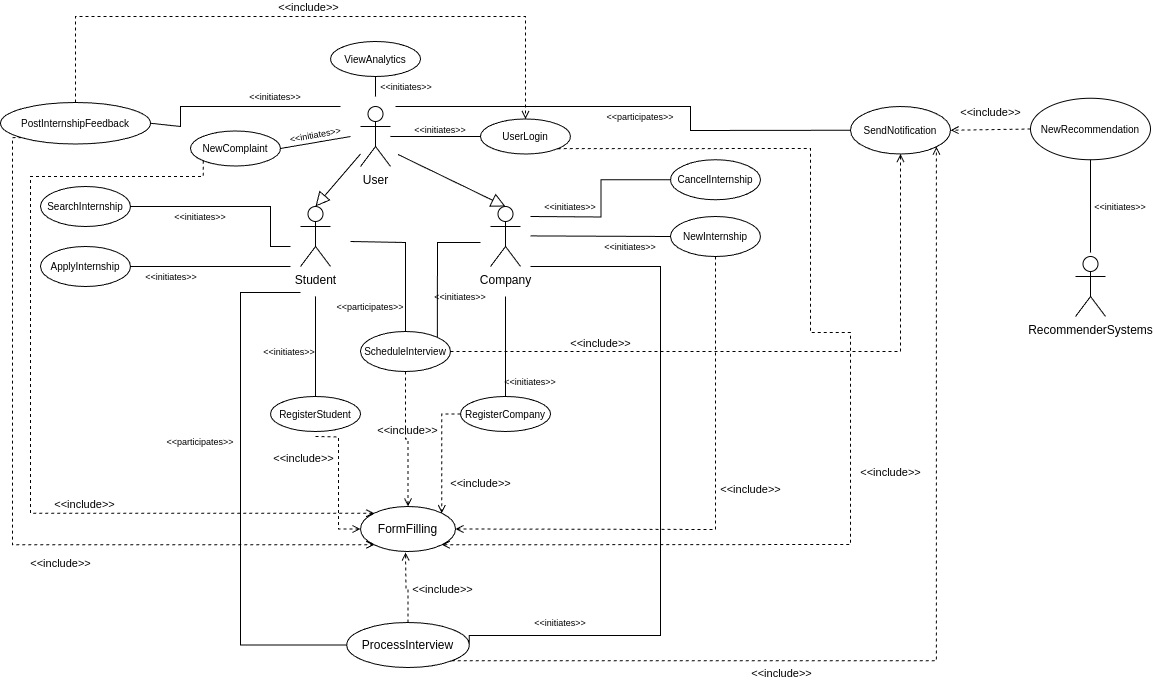
\includegraphics[width=\textwidth]{Images/use_case_diagram.png}
\caption{\label{fig:use-case-diagram} Use Case Diagram}
\end{figure}

\clearpage
\subsubsection{Sequence Diagrams}

\textbf{UC5: Search Internship} (Figure \ref{fig:search_sequence})
\begin{figure}[H]
\centering
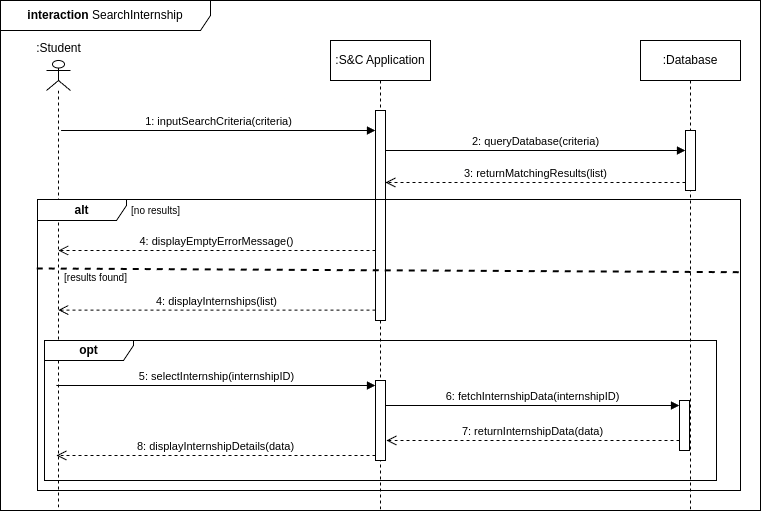
\includegraphics[width=\textwidth]{Images/searchInternship_sequence.png}
\caption{\label{fig:search_sequence} Search Internship Sequence Diagram}
\end{figure}

\textbf{UC7: New Recommendation} (Figure \ref{fig:matchmaking})
\begin{figure}[H]
\centering
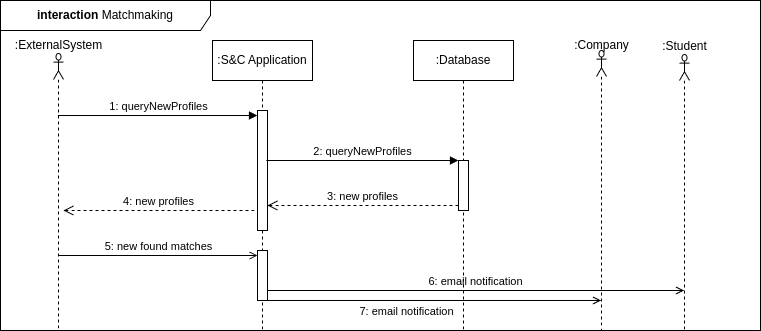
\includegraphics[width=\textwidth]{Images/matchmaking_sequence.png}
\caption{\label{fig:matchmaking} New Recommendation Sequence Diagram}
\end{figure}



\textbf{UC10: Schedule Interview} (Figure \ref{fig:schedule_sequence})
\begin{figure}[H]
\centering
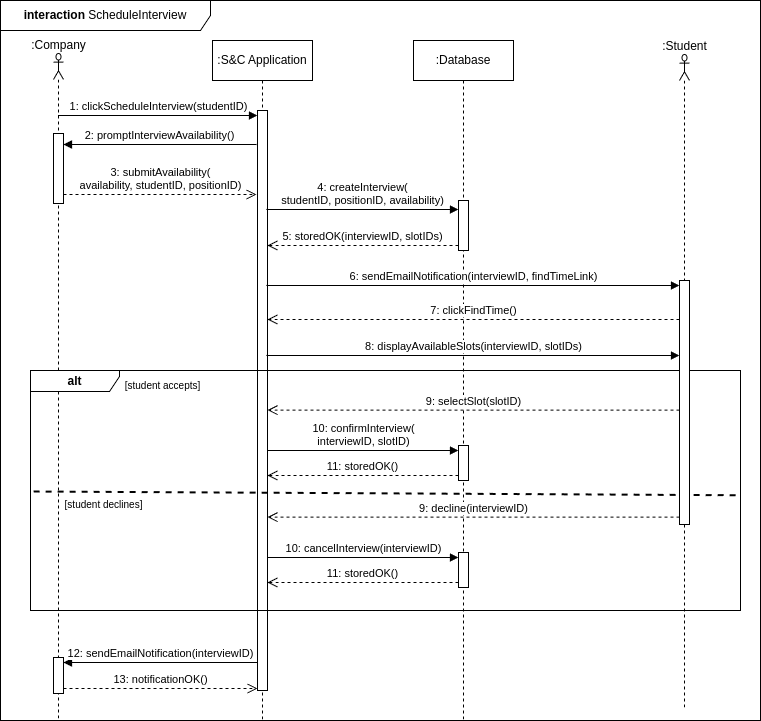
\includegraphics[width=\textwidth]{Images/schedule-interview_sequence.png}
\caption{\label{fig:schedule_sequence} Schedule Interview Sequence Diagram}
\end{figure}

\textbf{UC11: Process Interview} (Figure \ref{fig:process_sequence})
\begin{figure}[H]
\centering
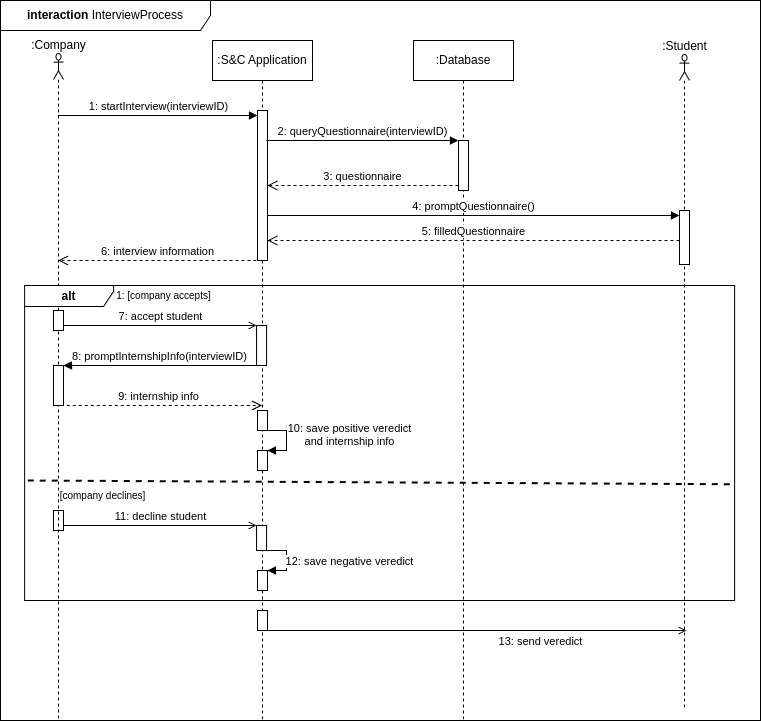
\includegraphics[width=\textwidth]{Images/interview_process_sequence.png}
\caption{\label{fig:process_sequence} Process Interview Sequence Diagram}
\end{figure}

\subsubsection{Activity Diagram}
We chose to include this activity diagram because it captures the complete end-to-end selection process on the S\&C platform. It highlights the interactions between the system, a single student, and a single company, illustrating how these parties engage throughout the application, interview, and internship stages.

This diagram emphasizes the interconnectedness of actions and decisions, providing a clear view of how the system facilitates and supports each step. By focusing on this interaction, we aim to provide readers with an intuitive understanding of the process and its flow, making the platform's functionality more transparent and comprehensible.

\begin{figure}[H]
\centering
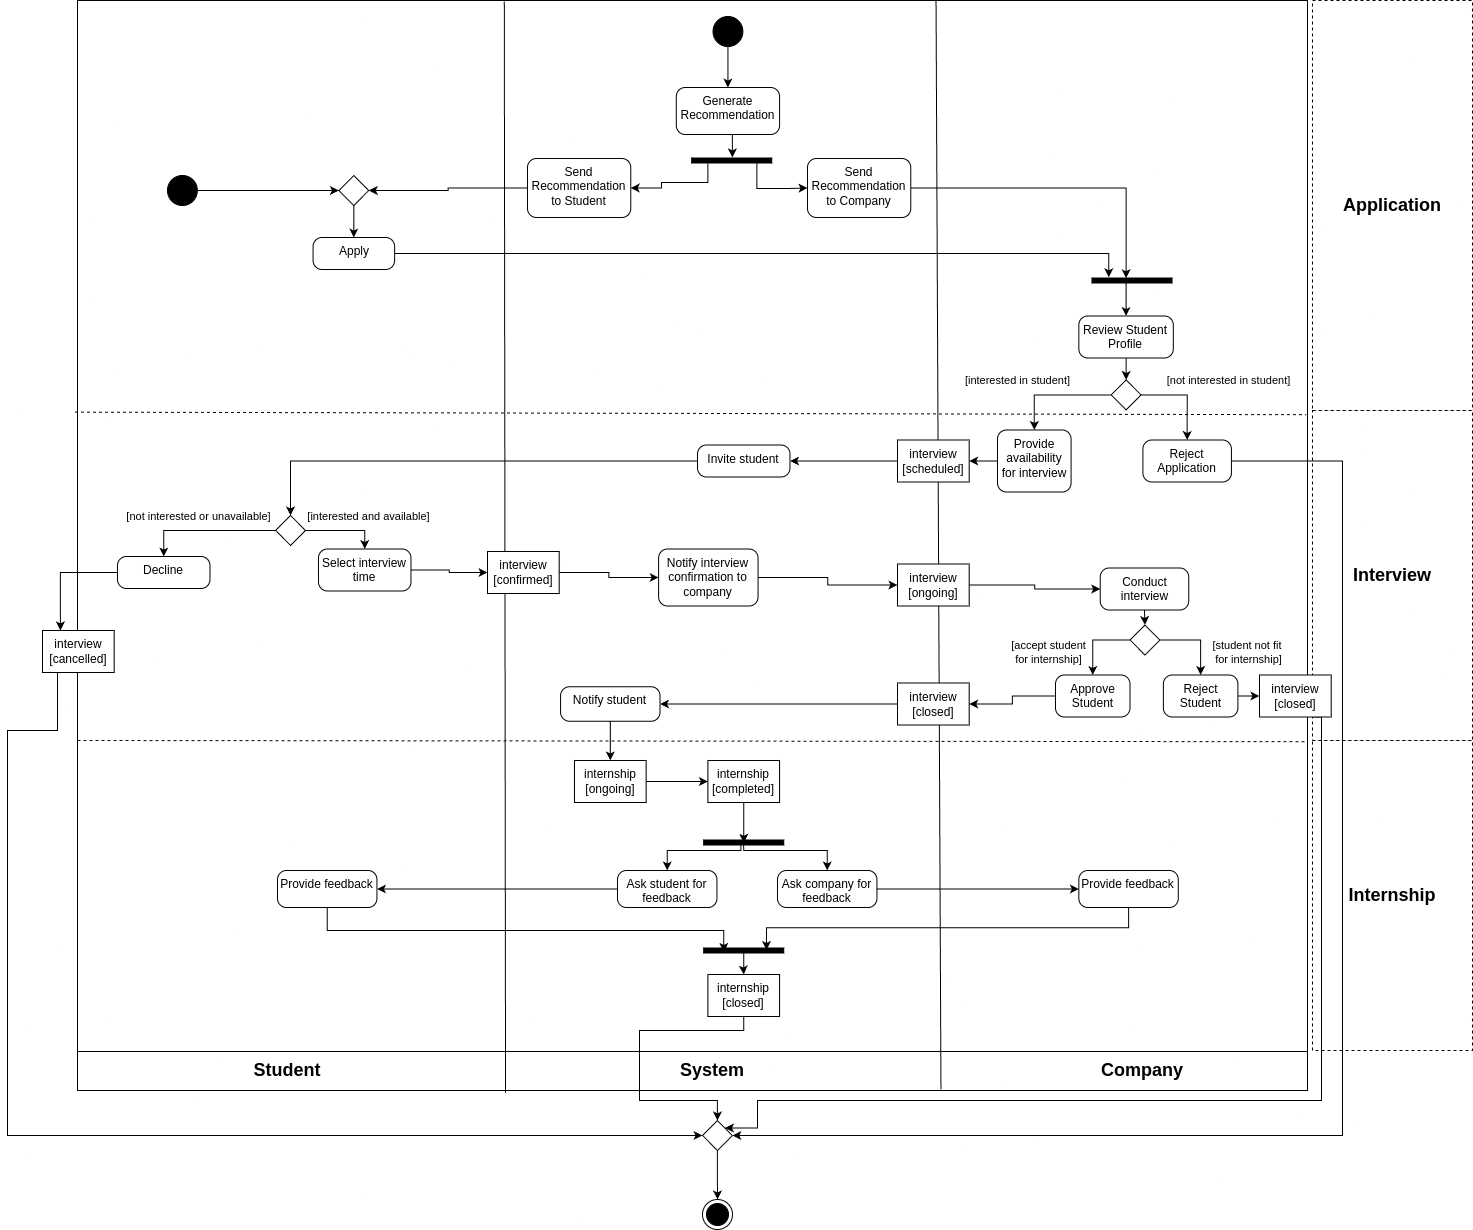
\includegraphics[width=\textwidth]{Images/activity-diagram.png}
\caption{\label{fig:activity_diagram} Activity Diagram}
\end{figure}


\subsubsection{Requirement Mapping}
\textbf{G1: Students are able to look for internships and easily recognize the ones that match their characteristics (skills, interests, experience…)} (Table \ref{tab:g1_Req_mapping})

\begin{table}[H]
\centering
\begin{tabular}{|p{6cm}|p{6cm}|} \hline
\textbf{Requirements} & \textbf{Domain Assumptions} \\
\hline
\begin{tabular}[c]{@{}l@{}}{[}R2{]} When a student registers, the \\ system generates a profile containing \\ their experience, skills, and education.\\ \\ {[}R5{]} When an internship is successfully \\ created, the system generates a work \\ profile containing the required \\ experience and skills for the position.\\ \\ {[}R6{]} When an internship is successfully \\ created, it should be findable through \\ the search internship feature and \\ allow student applications. \\ \\ {[}R8{]} When an internship is \\ selected, the system’s user \\ interface summarizes internship \\ information. \\ \\{[}R9{]} When a student searches for \\ an internship through the platform, \\ the displayed internships are \\ within the selected filters. \\ \\{[}R10{]} When a student searches for \\ an internship through the platform, \\ the displayed internships are \\ ordered accordingly to the field \\ specified in student’s criteria. \\ \\{[}R11{]} The system shall allow students \\ to apply to the displayed internship \\ without adding additional information. \\ \\{[}R12{]} When the application button is \\ clicked, the system shall save the \\ student information and profile and \\ notify the company. \end{tabular}
& \begin{tabular}[c]{@{}l@{}}D1: users provide accurate and \\ up-to-date information to the platform. \\ \\ D2: Students have a CV and a \\ notion of their skills and profile. \\ \\ D3: companies have a detailed notion \\ of the internship position and the \\ profile they are hiring for. \\ \\ D11: users remember their \\authentication info.\end{tabular} \\
\hline
\end{tabular}

\caption{G1 Requirements and Domain Assumptions}
\label{tab:g1_Req_mapping}
\end{table}

\textbf{G2: Companies are able to advertise their open internship projects and easily asses candidates’ fit with them}
(Table \ref{tab:g2_Req_mapping})
\begin{table}[H]
\centering
\begin{tabular}{|p{6cm}|p{6cm}|} \hline
\textbf{Requirements} & \textbf{Domain Assumptions} \\
\hline
\begin{tabular}[c]{@{}l@{}}{[}R1{]} The system should \\ provide authentication so \\ that each action can be \\ correctly associated with \\ a user. \\ \\ {[}R3{]} The system allows \\ companies to create new \\ internship positions at \\ any time. \\ \\ {[}R4{]} When a company user \\ clicks on “create internship”, \\ the system prompts the \\ company for all the required \\ information and checks its \\ validity before saving. \\ \\ {[}R5{]} When an internship is \\ successfully created, the system \\ generates a work profile \\ containing the required experience \\ and skills for the position. \\ \\ {[}R6{]} When an internship is \\ successfully created, it should \\ be findable through the search \\ internship feature and allow \\ student applications. \\ \\ {[}R17{]} The system allows \\ company users to review \\ any student profile. \\ \\ {[}R19{]} The system notifies the \\ company when there are new \\ student profiles to review \\ (either applied or \\ recommended).\end{tabular}
& \begin{tabular}[c]{@{}l@{}}D1. Users provide accurate \\ and up-to-date information \\ to the platform. \\ \\ D3. Companies have a detailed \\ notion of the internship position \\ and the profile they are hiring \\ for. \\ \\ D5. Students have a CV and a \\ notion of their skills and profile. \\ \\ D10. Students are proactively \\ interested in getting an \\ internship.\end{tabular} \\
\hline
\end{tabular}

\caption{G2 Requirements and Domain Assumptions}
\label{tab:g2_Req_mapping}
\end{table}


\textbf{G3: Students and companies are able to seamlessly communicate on topics related to the internship (questions, interviews, selection process, feedback)} (Table \ref{tab:g3_Req_mapping})


\begin{table}[H]
\centering
\begin{tabular}{|p{6cm}|p{6cm}|} \hline
\textbf{Requirements} & \textbf{Domain Assumptions} \\
\hline
\begin{tabular}[c]{@{}l@{}}{[}R1{]} The system should \\ provide authentication so \\ that each action can be \\ correctly associated with \\ a user. \\ \\ {[}R11{]} The system shall allow \\ students to apply to the \\ displayed internship without \\ adding additional information. \\ \\ {[}R12{]} When the application \\ button is clicked, the system \\ shall save the student \\ information and profile and \\ notify the company. \\ \\ {[}R18{]} The system allows \\ company users to invite \\ any student to an interview. \\ \\ {[}R20{]} When the company user \\ clicks on “invite to interview” \\ over a student, the system \\ prompts the company user to \\ provide possible availability \\ slots for that specific interview. \\ \\ {[}R21{]} When the company user \\ creates an interview by providing \\ their availability, the system \\ notifies the selected student \\ in less than 6 hours after the \\ interview creation.\end{tabular}
& \begin{tabular}[c]{@{}l@{}}D1. Users provide accurate \\ and up-to-date information \\ to the platform. \\ \\ D4. Internships are temporal \\ contracts with explicit \\ deadlines. \\ \\ D5. Companies have a pre-defined \\ process for hiring that involves \\ interaction with students \\ and companies. \\ \\ D6. The company user sticks to \\ the company-defined hiring \\ process through the platform. \\ \\ D7. Users interested in setting-up \\ interviews know in advance \\ their availability for the week. \\ \\ D8. Every user has a valid email \\ account that they check at least \\ once every 48 hours. \\ \\ D9. Email communication is \\ regarded by users as a \\ reliable channel for work-related \\ information.\end{tabular} \\
\hline
\end{tabular}
\caption{G3 Requirements and Domain Assumptions}
\label{tab:g3_Req_mapping}
\end{table}

\textbf{G4: Through tailored recommendations, students can find suitable internships when those exist}
(Table \ref{tab:g4_Req_mapping})

\begin{table}[H]
\centering
\begin{tabular}{|p{6cm}|p{6cm}|} \hline
\textbf{Requirements} & \textbf{Domain Assumptions} \\
\hline
\begin{tabular}[c]{@{}l@{}}{[}R2{]} When a student registers, \\ the system generates a profile \\ containing their experience, \\ skills, and education. \\ \\ {[}R3{]} The system shall attempt to \\ match student profiles with internship \\ profiles. \\ \\ {[}R5{]} When an internship is \\ successfully created, the system \\ generates a work profile \\ containing the required experience \\ and skills for the position. \\ \\ {[}R13{]} The system shall provide \\ regular monitoring to all stored \\ profiles from students and internships. \\ \\ {[}R32{]} When the duration time \\ of an internship has passed \\ since its starting time, the system \\ notifies and prompts both the \\ company user and the student \\ to provide feedback on the \\ internship experience. \\ \\ {[}R33{]} The system will not allow \\ any user to use other features \\ of the platform (besides login \\ and feedback) when they have \\ pending feedback on past internships. \\ \\  \\   \end{tabular}
& \begin{tabular}[c]{@{}l@{}}D2. Students have a CV and a \\ notion of their skills and profile. \\ \\ D3. Companies have a detailed \\ notion of the internship position \\ and the profile they are hiring for. \\ \\ D9. Email communication is \\ regarded by users as a \\ reliable channel for work-related \\ information. \\ \\ D11. Users remember their \\ authentication info. \end{tabular} \\
\hline
\end{tabular}
\caption{G4 Requirements and Domain Assumptions}
\label{tab:g4_Req_mapping}
\end{table}


\textbf{G5: Through tailored recommendations, companies can identify fitting candidates when those exist}
(Table \ref{tab:g5_Req_mapping})
\begin{table}[H]
\centering
\begin{tabular}{|p{6cm}|p{6cm}|} \hline
\textbf{Requirements} & \textbf{Domain Assumptions} \\
\hline
\begin{tabular}[c]{@{}l@{}}{[}R2{]} When a student registers, \\ the system generates a profile \\ containing their experience, \\ skills, and education. \\ \\ {[}R3{]} The system shall attempt to \\ match student profiles with internship \\ profiles. \\ \\ {[}R5{]} When an internship is \\ successfully created, the system \\ generates a work profile \\ containing the required experience \\ and skills for the position. \\ \\ {[}R13{]} The system shall provide \\ regular monitoring to all stored \\ profiles from students and internships. \\ \\ {[}R32{]} When the duration time \\ of an internship has passed \\ since its starting time, the system \\ notifies and prompts both the \\ company user and the student \\ to provide feedback on the \\ internship experience. \\ \\ {[}R33{]} The system will not allow \\ any user to use other features \\ of the platform (besides login \\ and feedback) when they have \\ pending feedback on past internships. \\ \\  \\   \end{tabular}
& \begin{tabular}[c]{@{}l@{}}D2. Students have a CV and a \\ notion of their skills and profile. \\ \\ D3. Companies have a detailed \\ notion of the internship position \\ and the profile they are hiring for. \\ \\ D9. Email communication is \\ regarded by users as a \\ reliable channel for work-related \\ information. \\ \\ D11. Users remember their \\ authentication info. \end{tabular} \\
\hline
\end{tabular}
\caption{G5 Requirements and Domain Assumptions}
\label{tab:g5_Req_mapping}
\end{table}


\subsection{Performance Requirements}

The \textit{Students\&Companies (S\&C)} platform is expected to handle high volumes of users, especially during peak times such as internship application seasons. Performance requirements include:
\begin{itemize}
  \item \textbf{Scalability}: The platform must support a growing number of students and companies without degradation in performance. This includes handling an increasing number of internship postings, student applications, and user interactions (e.g., profile creation, application submissions).
  \item {\textbf{Response Time}: User actions, such as searching for internships, submitting applications, or loading profiles, should be processed with a response time of less than 2 seconds to provide a seamless user experience.}
  \item \textbf{Concurrency}: The system should be capable of handling concurrent access by multiple users without performance bottlenecks, especially during high-traffic periods.
\end{itemize}

\subsection{Design Constraints}

\subsubsection{Standards Compliance}
The platform must adhere to relevant web development standards and best practices to ensure accessibility, compatibility, and security:
\begin{itemize}
  \item \textbf{Web Standards}: The platform will follow W3C standards for HTML, CSS, and JavaScript to ensure compatibility across different browsers and devices.
  \item \textbf{Accessibility}: The platform must be compliant with WCAG (Web Content Accessibility Guidelines) to ensure accessibility for users with disabilities.
  \item \textbf{Data Protection}: Compliance with GDPR (General Data Protection Regulation) and other relevant data privacy laws will be mandatory for managing user data, particularly personal and sensitive information.
\end{itemize}

\subsubsection{Hardware Limitations}
As a web-based platform, S\&C does not have specific hardware requirements beyond the devices that access the platform (computers, smartphones, etc.). However, the platform should be optimized to function smoothly on both different devices low-bandwidth connections.

\subsubsection{Other Constraints}
\begin{itemize}
  \item \textbf{Third-Party Services}: The platform relies on external APIs (such as email services and the recommendation engine), which must be available and integrated with the system to ensure seamless operations.
  \item \textbf{User Experience}: The platform should maintain an intuitive and user-friendly interface for both students and companies, ensuring ease of navigation and minimal training required.
\end{itemize}

\subsection{Software System Attributes}

\subsubsection{Reliability}
The platform must be reliable and fault-tolerant, with minimal downtime. Key reliability requirements include:
\begin{itemize}
  \item \textbf{Error Handling}: The system should handle user errors and system failures gracefully, providing informative error messages and recovery options where applicable.
  \item \textbf{Data Integrity}: The system must ensure data integrity, particularly for sensitive information such as student CVs and internship details. Automatic backup procedures will be in place to prevent data loss.
\end{itemize}

\subsubsection{Availability}
The platform should be highly available, aiming for 99.9\% uptime. This includes redundant servers and databases as well as load balancing among them.


\subsubsection{Security}
Security is critical given the personal and professional information handled by the platform. Security requirements include:
\begin{itemize}
  \item \textbf{Data Encryption}: All sensitive data, including student profiles and internship details, will be encrypted both in transit (using HTTPS) and at rest.
  \item \textbf{Authentication \& Authorization}: The platform will implement secure authentication mechanisms (e.g., OAuth, 2FA) for both students and companies to ensure that only authorized users can access sensitive features.
  \item \textbf{Access Control}: Different user roles (students, companies, universities) will have distinct access levels to ensure that users can only access information pertinent to their role.
\end{itemize}

\subsubsection{Maintainability}
The platform must be easy to maintain and update. This implies that the architecture, whichever is chosen further and specified in the design document, shall be modular enough to allow easy updates, bug fixes and feature addition. 

\subsubsection{Portability}
The platform should be portable across different operating systems and devices, ensuring accessibility for a wide range of users. This implies both cross-browser compatibility, to make sure it works seamlessly on many different browsers, and a design responsive enough to work on both desktop and mobile.



%------------------------------------------------------------------------------------------------------------------------------------------------
\clearpage
{\color{Blue}{\section{Formal Analysis Using Alloy}}}
\label{sect:alloy}
For the Alloy part we focused on the interview state machine, specially in the slot assignment process. The purpose of this choice was to ensure that the scheduling mechanism is consistent and to further explain its details.

First, we started with some signature definitions that helped us to properly define our model:

\lstinputlisting[language=alloy]{Files/alloy-code/signature-defs.tex}


Then, we moved on to some predicates to help us model and understand possible user actions that will trigger state transitions.

\lstinputlisting[language=alloy]{Files/alloy-code/predicates.tex}

Lastly, we wrote some facts to ensure the proper behavior of our model:

\lstinputlisting[language=alloy]{Files/alloy-code/facts.tex}

\subsection{Examples}

\begin{figure}[h]
\centering
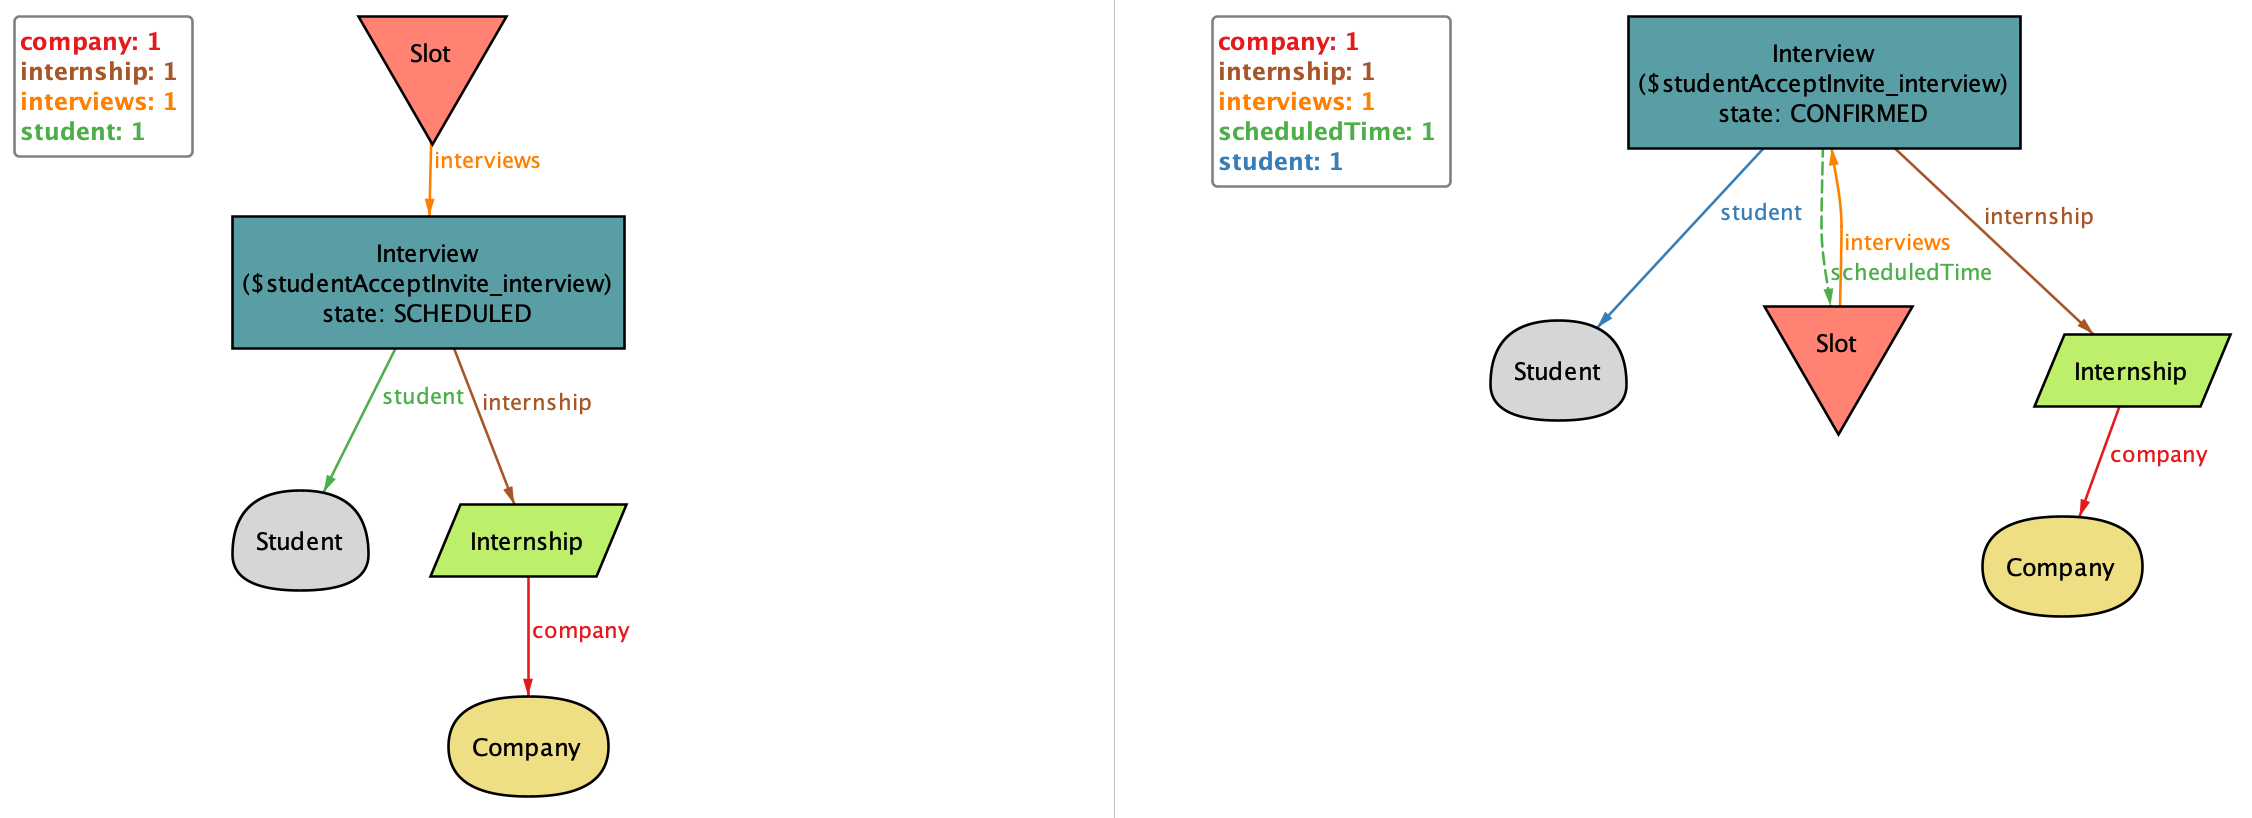
\includegraphics[width=\textwidth]{Images/caseOneInterview-1.png}
\caption{\label{fig:alloy-example-1-1} Example 1: One interview, steps 1 and 2}
\end{figure}

\begin{figure}[h]
\centering
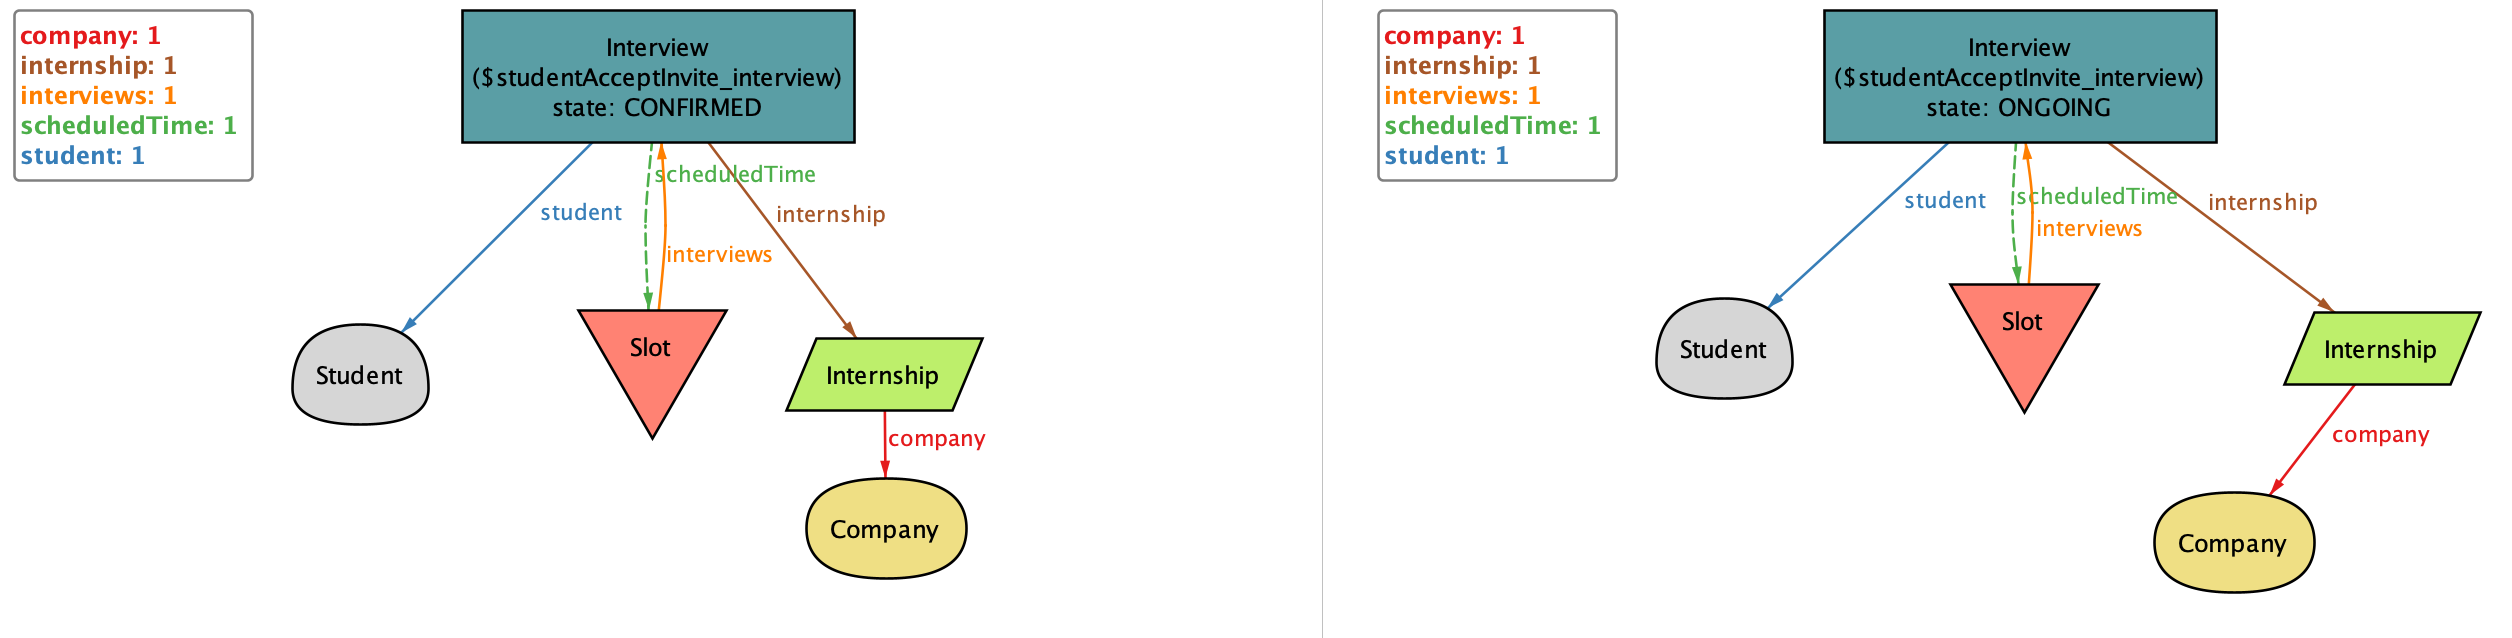
\includegraphics[width=\textwidth]{Images/caseOneInterview-2.png}
\caption{\label{fig:alloy-example-1-2} Example 1: One interview, steps 3 and 4}
\end{figure}

\begin{figure}[h]
\centering
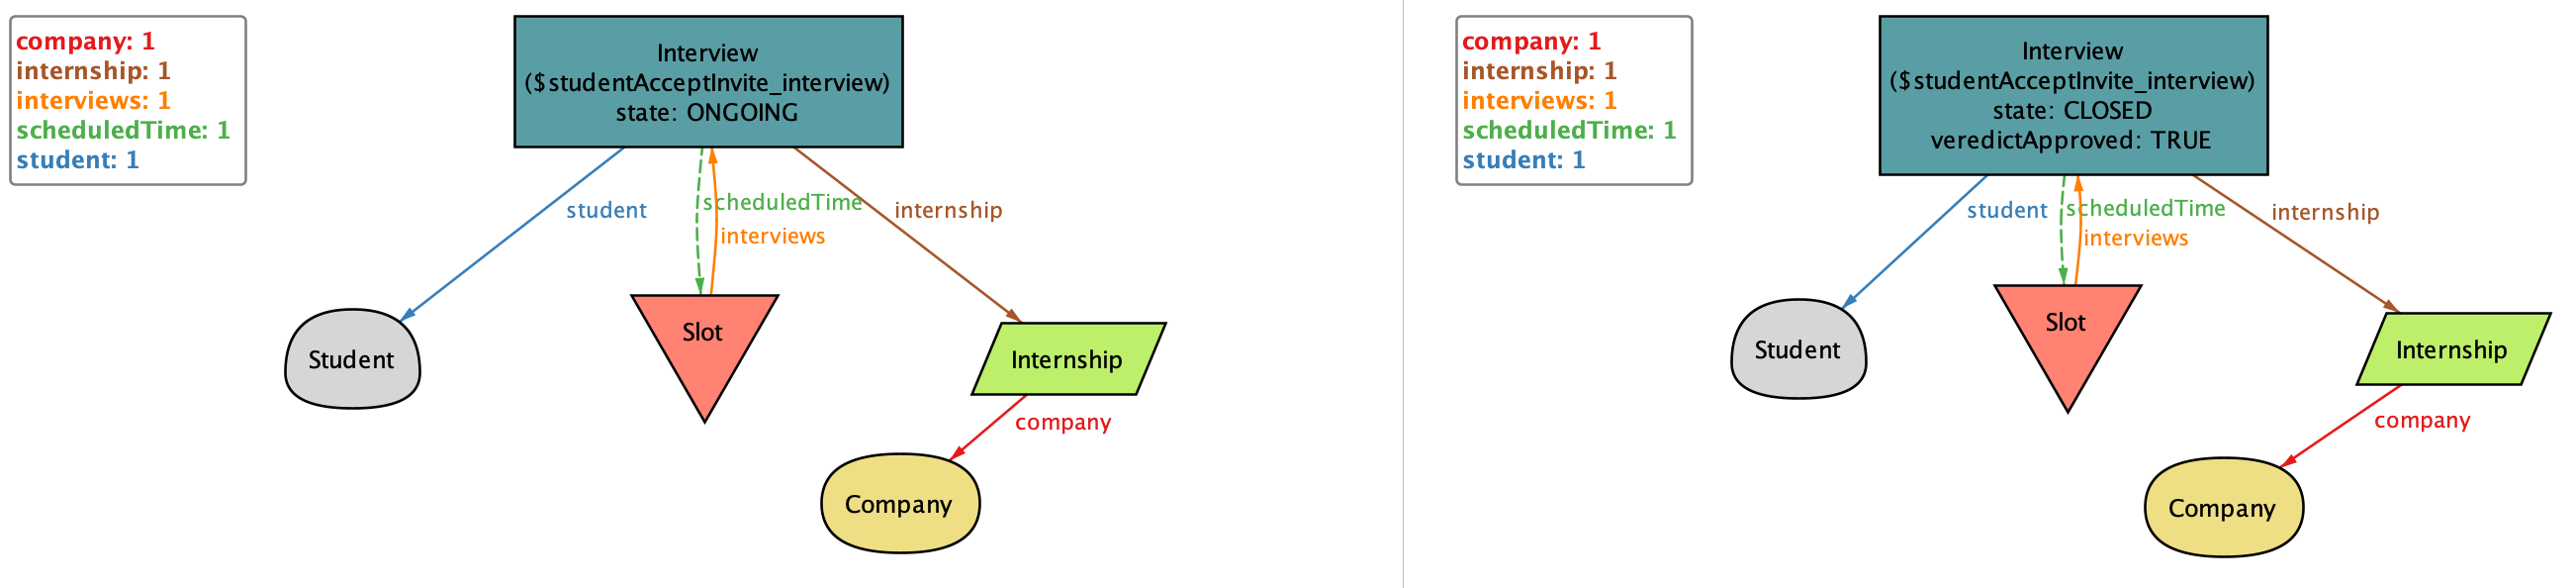
\includegraphics[width=\textwidth]{Images/caseOneInterview-3.png}
\caption{\label{fig:alloy-example-1-3} Example 1: One interview, steps 5 and 6}
\end{figure}

\begin{figure}[h]
\centering
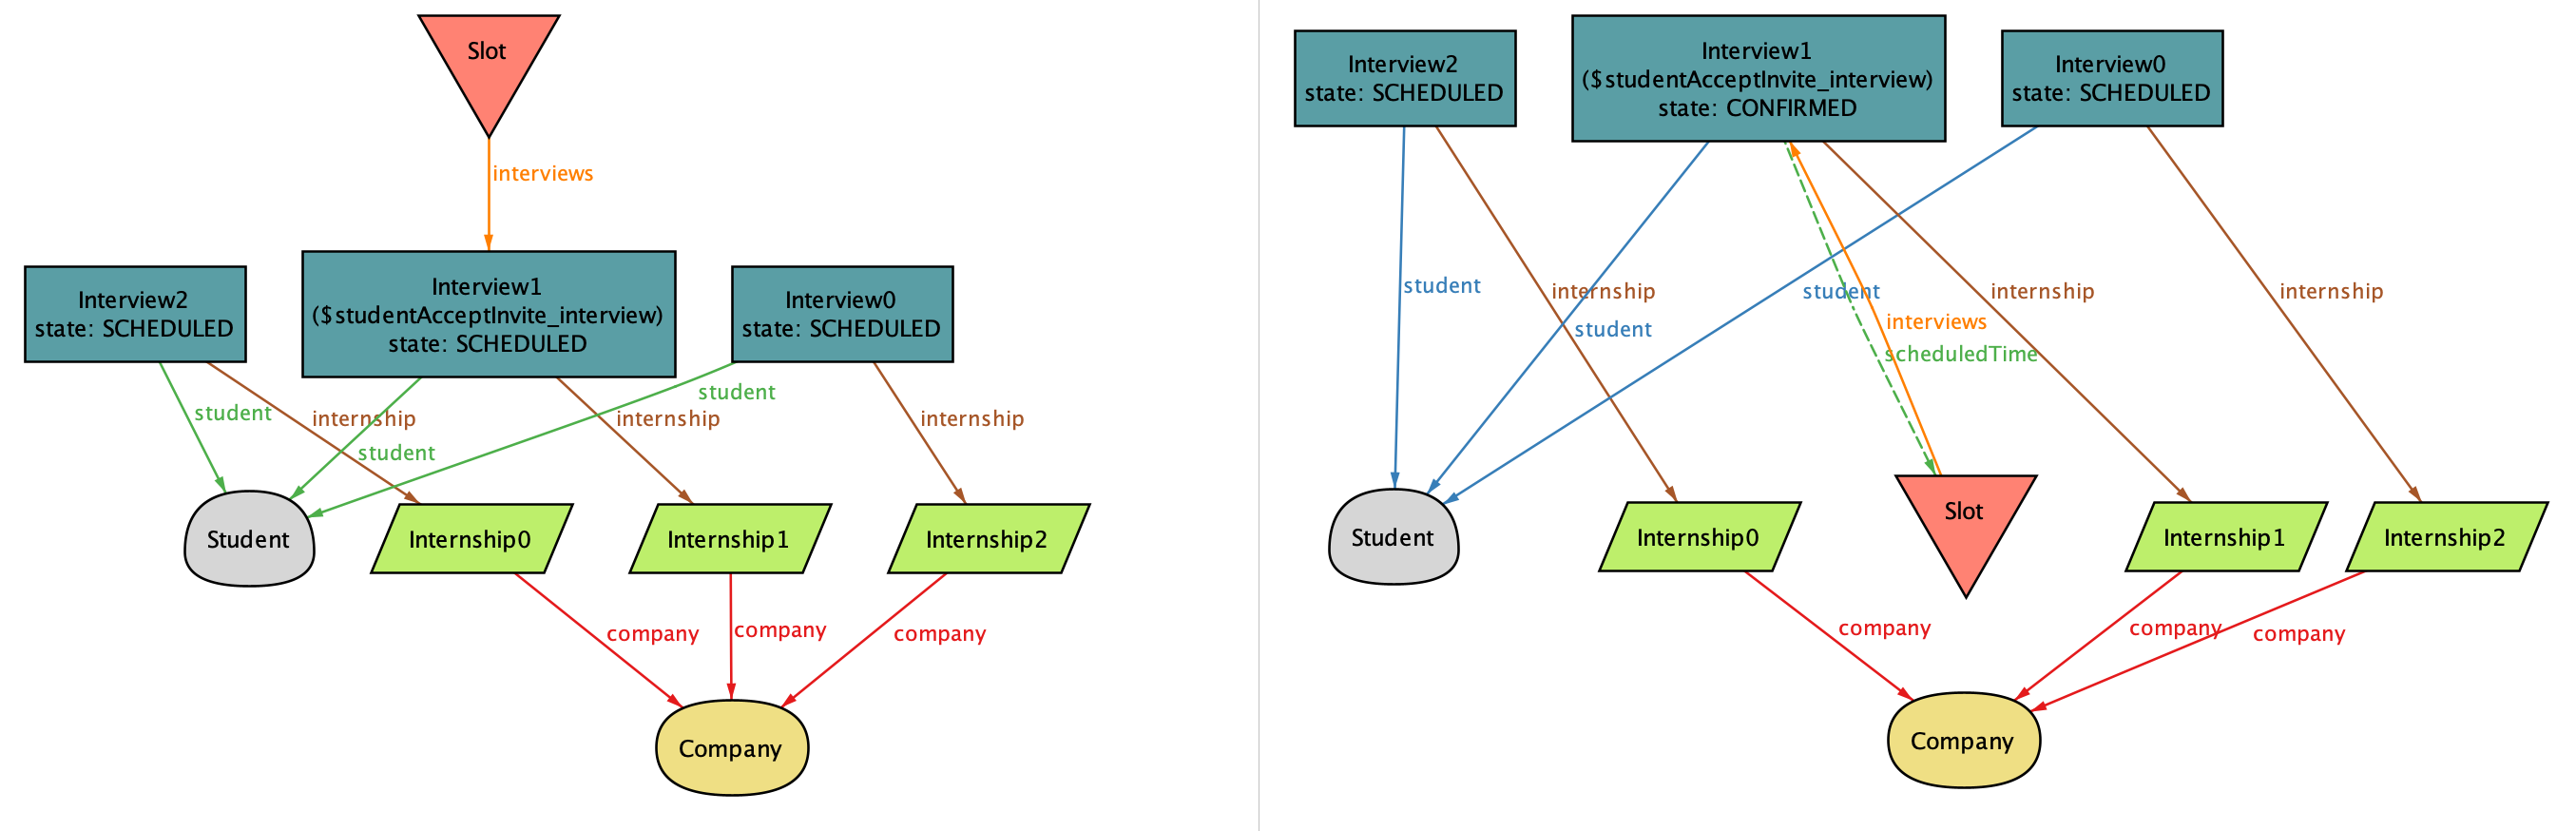
\includegraphics[width=\textwidth]{Images/caseThreeInterviews-1.png}
\caption{\label{fig:alloy-example-2-1} Example 2: Three interviews, steps 1 and 2}
\end{figure}

\begin{figure}[h]
\centering
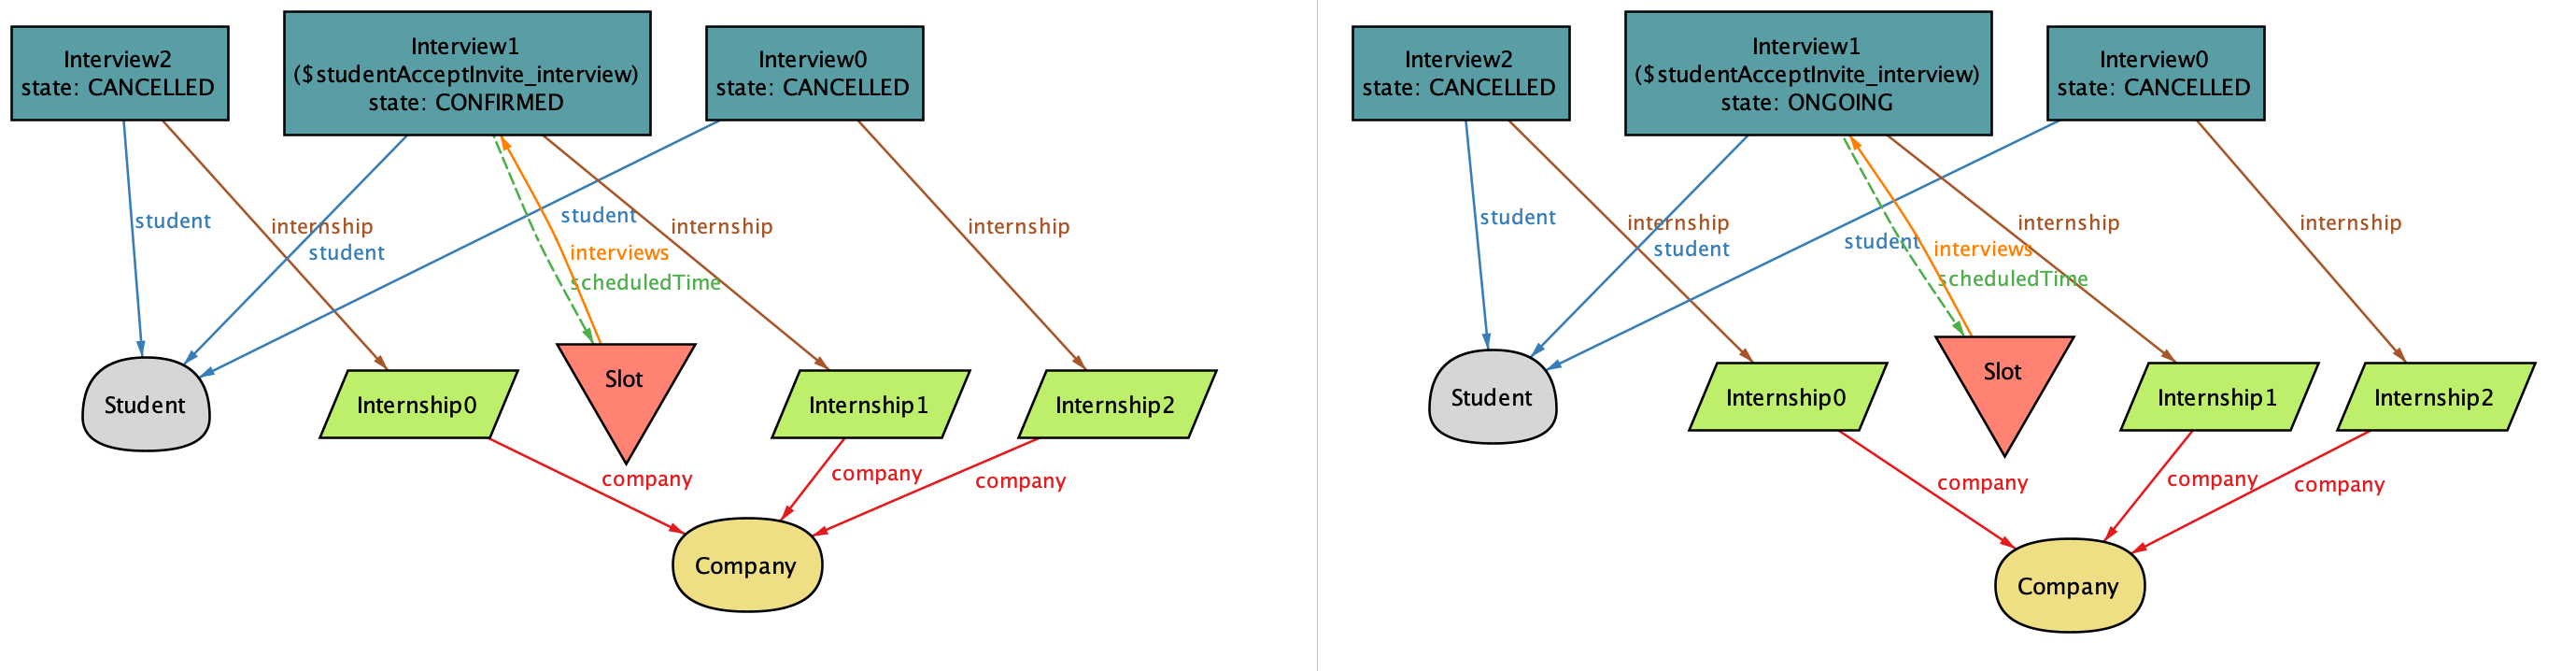
\includegraphics[width=\textwidth]{Images/caseThreeInterviews-2.png}
\caption{\label{fig:alloy-example-2-2} Example 2: Three interviews, steps 3 and 4}
\end{figure}

\begin{figure}[h]
\centering
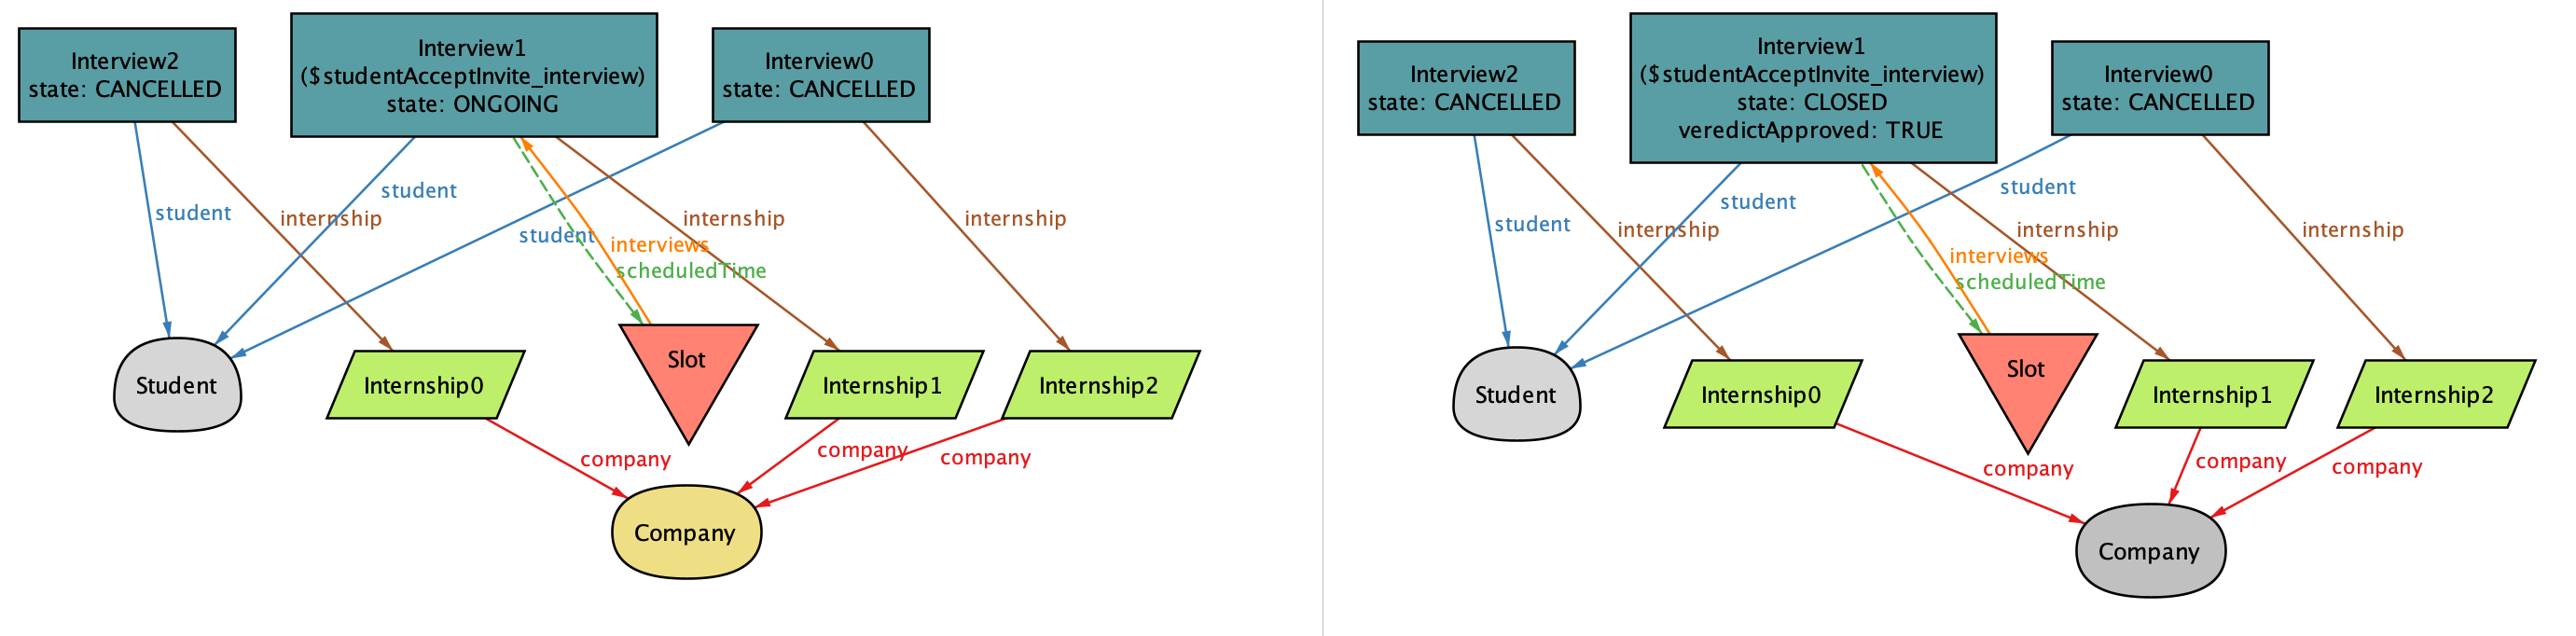
\includegraphics[width=\textwidth]{Images/caseThreeInterviews-3.png}
\caption{\label{fig:alloy-example-2-3} Example 2: Three interviews, steps 5 and 6}
\end{figure}

%------------------------------------------------------------------------------------------------------------------------------------------------
\clearpage
{\color{Blue}{\section{Effort Spent}}}
\label{sect:effort}
\begin{table}[H]
\centering
\begin{tabular}{|l|c|c|}
\hline
\textbf{Activity} & \textbf{Enzo (hours)} & \textbf{María (hours)} \\ \hline
Introduction & 6 & 6 \\ \hline
Overall Description & 8 & 7 \\ \hline
Specific Requirements & 9 & 8 \\ \hline
Formal Analysis Using Alloy & 7 & 9 \\ \hline
\end{tabular}
\caption{Hours dedicated to each activity by group members}
\label{tab:hours_dedication}
\end{table}



%------------------------------------------------------------------------------------------------------------------------------------------------
\clearpage
\addcontentsline{toc}{section}{References}
\bibliographystyle{plain}
\bibliography{main}
%------------------------------------------------------------------------------------------------------------------------------------------------




\end{document}
